\documentclass{article}

\usepackage{amsthm}

% !TeX TXS-program:compile = txs:///pdflatex/[--shell-escape]

\usepackage{amsfonts}
\usepackage{amsmath}
\usepackage{amssymb}
\usepackage{fullpage}
\usepackage[usenames]{color}
\usepackage{hyperref}
  \hypersetup{
    colorlinks = true,
    urlcolor = blue,       % color of external links using \href
    linkcolor= blue,       % color of internal links 
    citecolor= blue,       % color of links to bibliography
    filecolor= blue,        % color of file links
    }
    
\usepackage{listings}
\usepackage{minted}
\usepackage{graphicx}
\usepackage{pifont}
\usepackage{wrapfig}
\usepackage{enumitem}
\usepackage{indentfirst}

\setlist{noitemsep}

\definecolor{dkgreen}{rgb}{0,0.6,0}
\definecolor{gray}{rgb}{0.5,0.5,0.5}
\definecolor{mauve}{rgb}{0.58,0,0.82}
\definecolor{codeblue}{rgb}{0,0.3,0.6}
\newcommand{\mybluecode}[1]{%
{\color{codeblue}%
\mintinline[]{c++}{#1}}%
}
%\newmintline[bluecode]{c++}{\color{codeblue}}

\lstset{frame=tb,
  language=haskell,
  aboveskip=3mm,
  belowskip=3mm,
  showstringspaces=false,
  columns=flexible,
  basicstyle={\small\ttfamily},
  numbers=none,
  numberstyle=\tiny\color{gray},
  keywordstyle=\color{blue},
  commentstyle=\color{dkgreen},
  stringstyle=\color{mauve},
  breaklines=true,
  breakatwhitespace=true,
  tabsize=3
}

\theoremstyle{theorem} 
  \newtheorem{theorem}{Theorem}[section]
  \newtheorem{corollary}[theorem]{Corollary}
  \newtheorem{lemma}[theorem]{Lemma}
  \newtheorem{proposition}[theorem]{Proposition}
\theoremstyle{definition}
  \newtheorem{definition}[theorem]{Definition}
  \newtheorem{example}[theorem]{Example}
\theoremstyle{remark}    
  \newtheorem{remark}[theorem]{Remark}


\title{CPSC-354 Report}
\author{Natalie Huante  \\ Chapman University}

\date{\today}

\begin{document}

\maketitle

\begin{abstract}
This report was made for my personal reflections on the Fall 2023 Programming Languages course, taught by Professor Alexander Kurz. 
It contains both material from the semester along with a series of my personal reflections and a couple extra details.
\end{abstract}

\tableofcontents

\section{Introduction}\label{intro}

This report was made for my personal reflections on the Fall 2023 Programming Languages course, taught by Professor Alexander Kurz. It includes all of our homework assignment, 
along with my thoughts or my process for completing them, my thoughts on the project I developed and a few extra details. For all of the homework assignments, my goal was to 
review the concepts we learned in lecture and explain them in my own understanding as well as how they relate to the assignment. My goal was to not only include the technical
 answers but also explain my thinking in finding the solution. 


My project was developed throughout the entirety of the semester and by a team of three (myself, Kyle, and Lauren). 
\href{https://github.com/KyleWynne/Health_Blocks}{You can see the repository for the project here.}
This project was made in the effort to create a more accessible and intuitive method for users to access a nutritional database without the need for previous experience using 
an API. We used both the Nutritionix API's database and natural language processing model alongside the Blockly API in order to create our final product. For anyone interested, 
the project's repository gives a much more detailed description and explanation behind its implementation. 


This document was developed in LaTeX and, along with the Health Blocks project,  makes up the bulk of the coursework for the class. Lastly, this report is not merely an 
accumulation of the work from the semester, but rather a more polished version of what I have learned from each lecture and assignment as well as from the course as a whole. 

\section{Homework}\label{homework}
This section contains solutions to homework. For each assignment, my goal was to review the concepts we learned in lecture and explain them in my own understanding 
as well as how they relate to the assignment. My goal was to not only include the technical answers but also explain my thinking in finding the solution. This was 
particularly helpful for me to do because it forced me to go back and review the concepts from lecture so that I could develop a good enough understanding to then 
be able to write about it in my own words. 


\subsection{Week 1}

The homework for Week 1 is dedicated to allow myself the opportunity to get familiar with LaTeX as well as review the model of equational reasoning. 
In this lesson, we used the Fibonacci Sequence as an example of this, but we will use the function of Greatest Common Divisor for the assignment.
In terms of familiarity with LaTeX, I do have experience through the Algorithm Analysis report from the previous 
semester (Spring 2023). However, this serves as a way to remind myself of the language and it's syntax. \\


For context, the definition the GCD function is as follows:\\
\noindent
  {\color{gray} \rule{\linewidth}{0.05mm}}
\begin{center}
  \begin{verbatim}
  gcd(a,b): 
  Input: Two whole numbers (integers) called a and b, both greater than 0.
  (1) if a>b then replace a by a-b and go to (1).
  (2) if b>a then replace b by b-a and go to (1).
  Output: a
  \end{verbatim}
\end{center}
\noindent
  {\color{gray} \rule{\linewidth}{0.05mm}}

Now, I will write out the full computation of gcd(9,33) below:

\begin{align*}
  gcd(9,33) & = gcd(9,24)\\
            & = gcd(9,15)\\
            & = gcd(9,6)\\
            & = gcd(3,6)\\
            & = gcd(3,3)\\
            & = 3
\end{align*}


As you can see above, the basis of the function is to iteratively decrement a and b until you reach a point at which you can no longer
decrement them by the definition given. Once you reach this point, it will indicate that you have calculated the greatest common divisor, which 
in this case is 3. When a and b are both equal to 3 in this example, or equal to eachother in a broader case, then neither rule 1 or 2 will apply to them. This means you can no longer 
continue to rewrite the equation and you have reached the end result. 

\subsection{Week 2}
For this week's homework we wil take a look back at and view some practice examples based on our discussion of the Towers of Hanoi problem. To solve the Towers of Hanoi one must move all the rings
from the left-most tower to the right-most tower. However, discs can only be placed on other discs larger than themselves. Therefore, we have to logically think about the 
order in which we move them as well as how we can most efficiently do so (aka in the least amount of moves). I have included a visual representation of what this problem looks like below: 
\begin{center}
  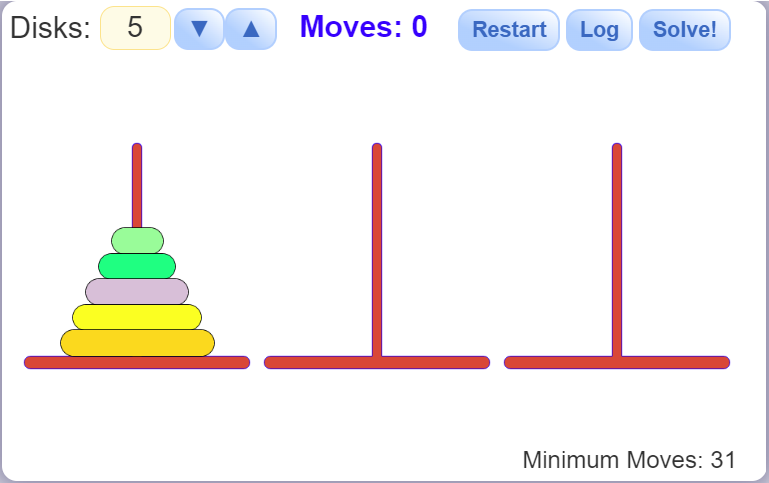
\includegraphics[scale=0.7]{towersOfHanoi_visual.png}
\end{center}

In our class discussion, we established a set of rules in order to then discuss how to represent our functions in code. Below I include both rules as well as repeat some notes on notation 
in order to allow for some context on the second half of this assignment.\\
\noindent
  {\color{gray} \rule{\linewidth}{0.05mm}}
\begin{center}
  \begin{minted}{haskell}
    // Rules
    hanoi 1 x y = move x y 

    hanoi (n+1) x y = 
      hanoi n x (other x y)
      move x y 
      hanoi n (other x y) y
  \end{minted}
\end{center}
\noindent
  {\color{gray} \rule{\linewidth}{0.05mm}}

Notes on notation: 
\begin{itemize}
  \item read \mintinline{haskell}{hanoi n x y} as "move tower of n disks from x to y"
  \item think about how to move a tower of n+1 disks assuming we already know how to move a tower of n disks 
  \item \mintinline{haskell}{hanoi n x y} is a function that takes three arguments: a number n (the number of disks), a number x (encoding the place where the tower is, a number y (encoding the place
  where the tower should go))
  \item \mintinline{haskell}{move x y} is a function that moves one disk (the topmost disk) from x to y 
  \item \mintinline{haskell}{other x y} denotes the third place which is neither x nor y 
\end{itemize}

Now having laid down some rules for our discussion, we observed that the nature of the Towers of Hanoi problem is recursive, given that in order to solve a tower of 4 disks we must first solve 
it with 3 disks and then that requires we solve it for 2 disks and so on. In class, we observed the 5 disk tower solution or \mintinline{haskell}{hanoi 5 0 2}. For this assignment, I will write out the 
implementation of this function to cement what we learned about its recursion and logic. \\

\noindent
  {\color{gray} \rule{\linewidth}{0.05mm}}
\begin{minted}{haskell}
  hanoi 5 0 2
    hanoi 4 0 1
      hanoi 3 0 2
        hanoi 2 0 1
          hanoi 1 0 2 = move 0 2
          move 0 1
          hanoi 1 2 1 = move 2 1
        move 0 2
        hanoi 2 1 2 
          hanoi 1 1 0 = move 1 0 
          move 1 2
          hanoi 1 0 2 = move 0 2
      move 0 1
      hanoi 3 2 1 
        hanoi 2 2 0
          hanoi 1 2 1 = move 2 1 
          move 2 0
          hanoi 1 1 0 = move 1 0
        move 2 1
        hanoi 2 0 1
          hanoi 1 0 2 = move 0 2
          move 0 1
          hanoi 1 2 1 = move 2 1
    move 0 2
    hanoi 4 1 2
      hanoi 3 1 0
        hanoi 2 1 2
          hanoi 1 1 0 = move 1 0
          move 1 2
          hanoi 1 0 2 = move 0 2
        move 1 0
        hanoi 2 2 0
          hanoi 1 2 1 = move 2 1
          move 2 0
          hanoi 1 1 0 = move 1 0
      move 1 2
      hanoi 3 0 2
        hanoi 2 0 1
          hanoi 1 0 2 = move 0 2
          move 0 1
          hanoi 1 2 1 = move 2 1
        move 0 2
        hanoi 2 1 2
          hanoi 1 1 0 = move 1 0 
          move 1 2
          hanoi 1 0 2 = move 0 2
\end{minted}
\noindent
  {\color{gray} \rule{\linewidth}{0.05mm}}

As we can see, this is a very lengthy program that relies on its recursive nature to solve the hanoi problem. Now, if we extract from this execution the moves that solve the puzzle (in their right order), we will see that there are 31 moves for the 5-disk tower 
that will solve the problem most efficiently. I say that these are the steps that actually solve the problem since they are the ones that will prompt moving a disk from one tower to another. The remaining steps in the above program are used to determine which disk to move 
and from which position to which position. Anyways, I will rewrite the "solving" steps again below: \\

\noindent
  {\color{gray} \rule{\linewidth}{0.05mm}}
\begin{minted}{haskell}
  move 0 2
  move 0 1
  move 2 1
  move 0 2
  move 1 0
  move 1 2
  move 0 2
  move 0 1 
  move 2 1
  move 2 0
  move 1 0
  move 2 1
  move 0 2
  move 0 1
  move 2 1
  move 0 2
  move 1 0
  move 1 2
  move 0 2
  move 1 0
  move 2 1
  move 2 0
  move 1 0
  move 1 2
  move 0 2
  move 0 1
  move 2 1
  move 0 2
  move 1 0
  move 1 2
  move 0 2
\end{minted}
\noindent
  {\color{gray} \rule{\linewidth}{0.05mm}}

Now that we have written out the exection, we can also see that the word \mintinline{haskell}{hanoi} appears many times in the computation. I observed the number of occurrences and recorded them in the below table. By looking at the table, we can notice that the
number of occurrences can actually be represented as a formula, for they increase in the same intervals exponentially. Therefore, we can say that with n disks, the number of times the word \mintinline{haskell}{hanoi} appears in the computation is \(2^n - 1\). 
\begin{center}
  \begin{tabular}{|c c c|}
    \hline
    n disks & num of hanoi  & \(2^n - 1\)\\
    \hline 
    1 & 1 & \(2^1 - 1\)\\
    \hline 
    2 & 3 & \(2^2 - 1\)\\
    \hline 
    3 & 7 & \(2^3 - 1\)\\
    \hline 
    4 & 15 & \(2^4 - 1\)\\
    \hline 
    5 & 31 & \(2^5 - 1\)\\
    \hline
  \end{tabular}
\end{center}


\subsection{Week 3}
In this week's homework, we are reviewing parsing and context-free grammars. The concept of parsing is important to understand as we need it to translate concrete syntax (what we see as more human-readable) into abstract syntax (what a computer will see as more readable). 
In class, we focused on processing abstract syntax in a 2-dimensional view, or what resembles a tree. A context-free grammar is a set of rules that defines a language. One of the examples we used, and the one we will use for the following problems, is a context-free grammar that 
defines arithmetic expressions. In other words, a string is considered to be part of the language defined if it can be dervied from the rules below. \\
\noindent
  {\color{gray} \rule{\linewidth}{0.05mm}}
\begin{minted}{haskell}
  Exp -> Exp '+' Exp1
  Exp1 -> Exp1 '*' Exp2
  Exp2 -> Integer 
  Exp2 -> '(' Exp ')'
  Exp -> Exp1
  Exp1 -> Exp2
\end{minted}
\noindent
  {\color{gray} \rule{\linewidth}{0.05mm}}

Now that we have the rules above, I will write out the derivation trees (aka parse trees or conccrete syntax trees) for the following strings. Note that I numbered the rules above and wrote, in blue, the number of the rule used in each step. The integer definition is implied here so there is no 
number written next to those translations. 
\begin{itemize}
  \item[\ding{99}] 1. 2+1
  \item[\ding{99}] 2. 1+2*3
  \item[\ding{99}] 3. 1+(2*3)
  \item[\ding{99}] 4. (1+2)*3
  \item[\ding{99}] 5. 1+2*3+4*5+6
\end{itemize}

\begin{center}
  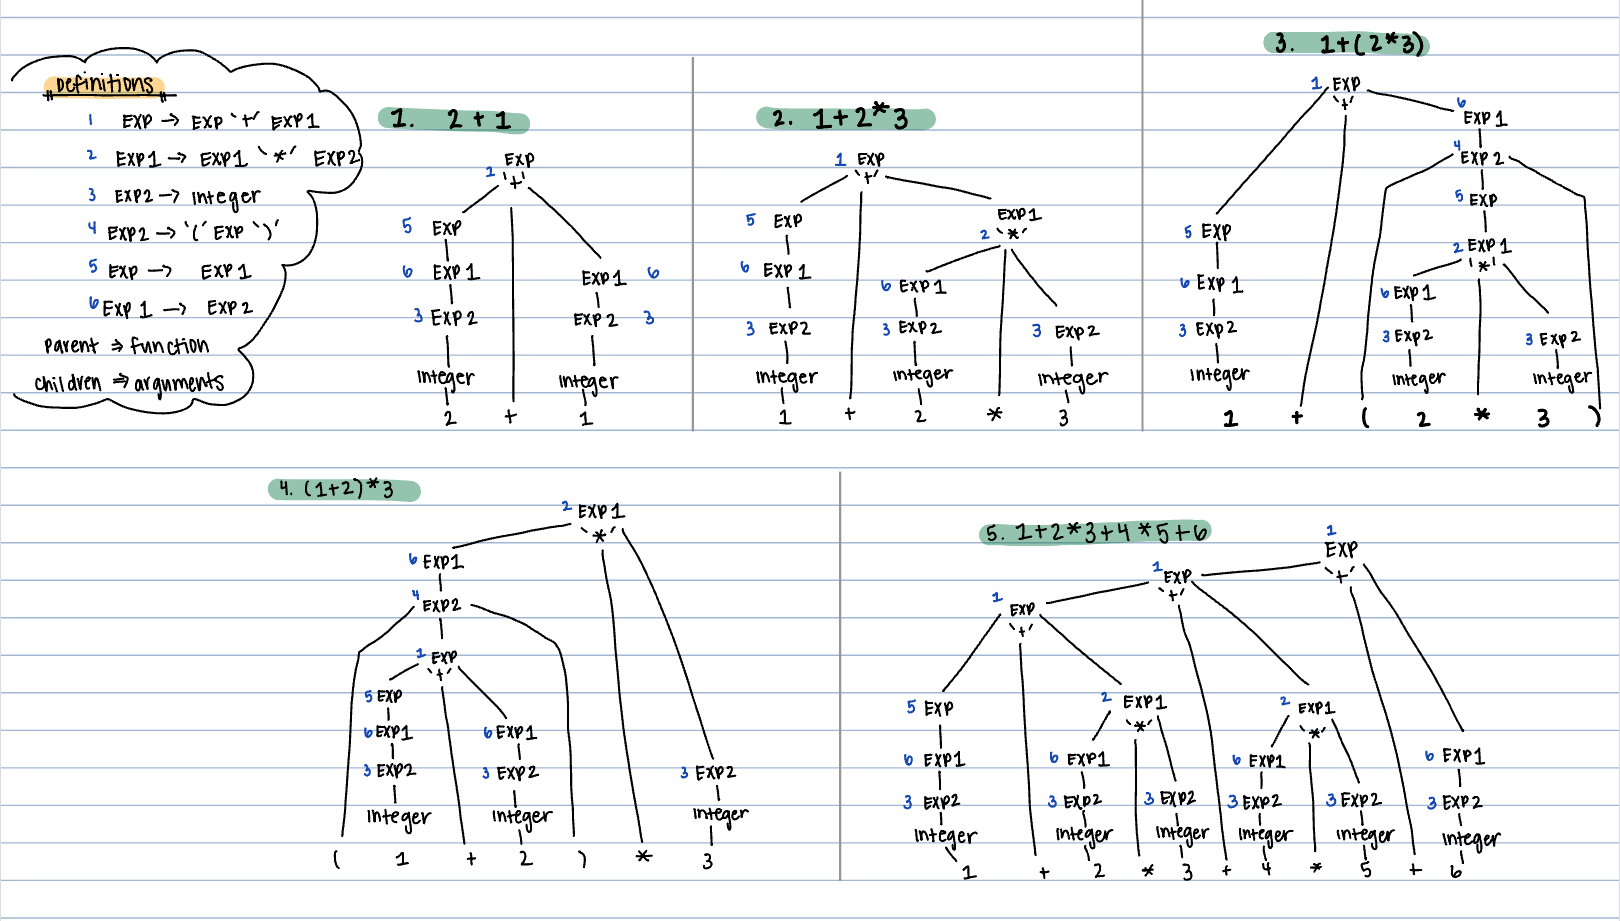
\includegraphics[scale=0.3]{parsing_arithmetic.jpg}
\end{center}

Now that we have covered what the parsing process looks like, we can think bigger. In other words, we can think of a parser that will automatically translate concrete syntax into abstract syntax. Looking back at our lecture, we do not attempt to create this type of parser ourselves, but rather 
used a parser generator. By this I mean that we will input a context-free grammer (like the one above) and the generator will output a parser.


To accomplish this, I first installed the parser generator BNFC, which proved to be a feat of its own. After multiple error messages and researching on the side, I was able to successfully download the generator as well as the necessary libraries (alex, happy, etc.). The first commands I used are those described in the 
lecture: 

\noindent
  {\color{gray} \rule{\linewidth}{0.05mm}}

\begin{minted}{haskell}
  bnfc -m -haskell numbers.cf
  make
  echo "1+2*3" | ./TestNumbers
\end{minted}

\noindent
  {\color{gray} \rule{\linewidth}{0.05mm}}


In short, the first two commands generated the parser and the third command ran the input "1+2*3 through the generated parser. 
The generation of the parser also created extra files needed and then the test input ran gave me the following output: 

\begin{center}
  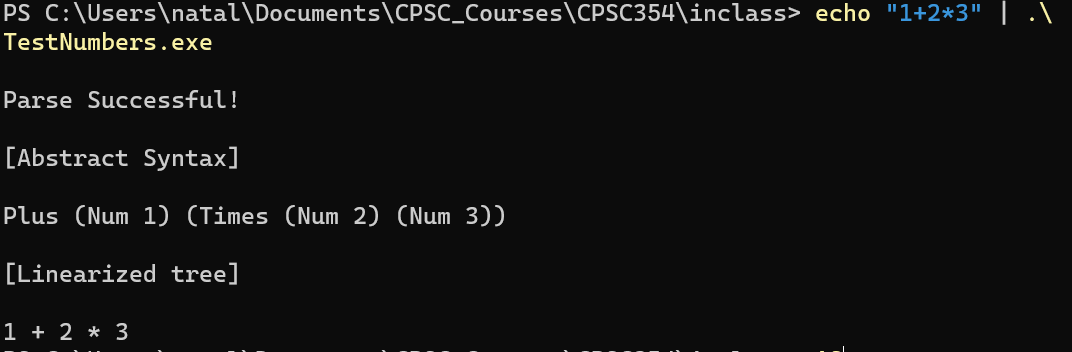
\includegraphics[width=15cm]{bnfc_intro_example.png}
\end{center}

As you can see, my test input is shown on the bottom and the abstract syntax tree is shown in the middle there. The input has been translated to fit into the syntax we wanted and has identified that the Times operation should be prioritized over the Plus operation. 
Having run the example successfully, I will now show the outputs for the following given strings: 

**You will note that these are the same exercises I translated by hand above**\\
\begin{center}
  \textbf{1. 2 + 1} \\
  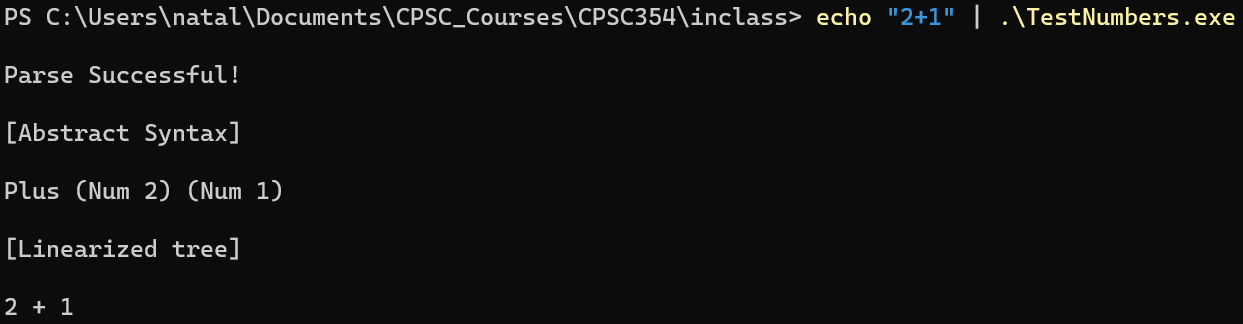
\includegraphics[width=15cm]{bnfc_exercise1a.png}

  \textbf{2. 1 + 2 * 3}\\
  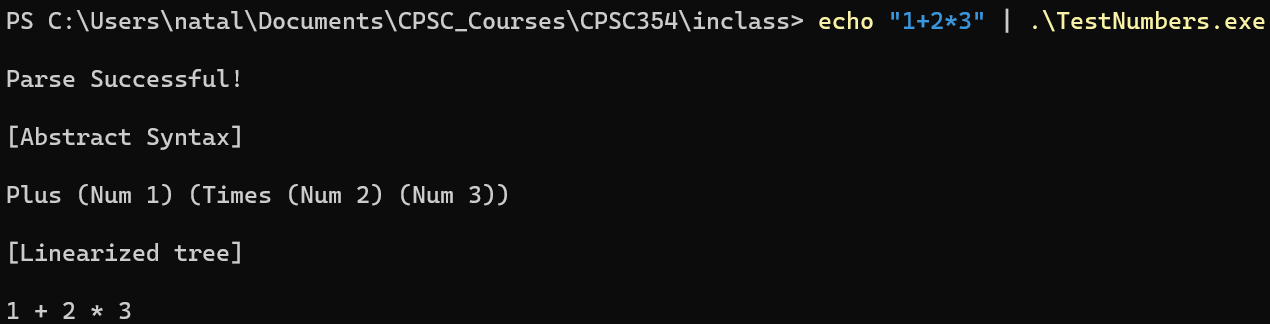
\includegraphics[width=15cm]{bnfc_exercise1b.png}

  \textbf{3. 1 + ( 2 * 3 )}\\
  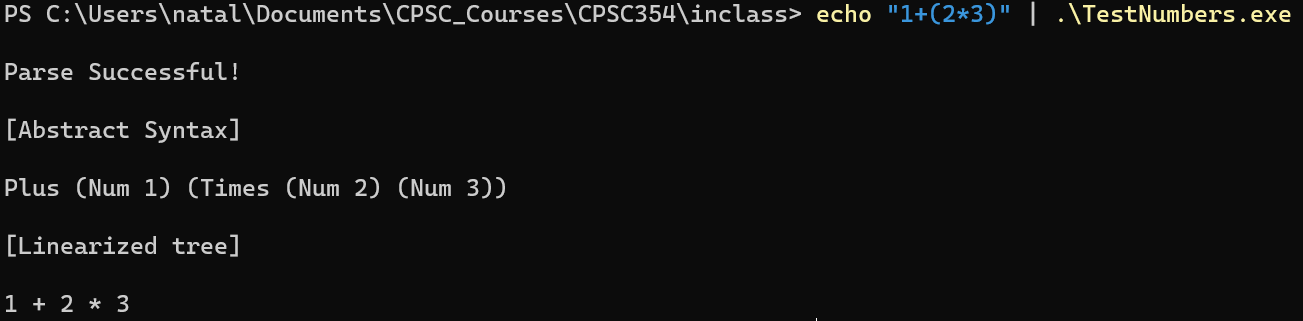
\includegraphics[width=15cm]{bnfc_exercise1c.png}

  \textbf{4. ( 1 + 2 ) * 3}\\
  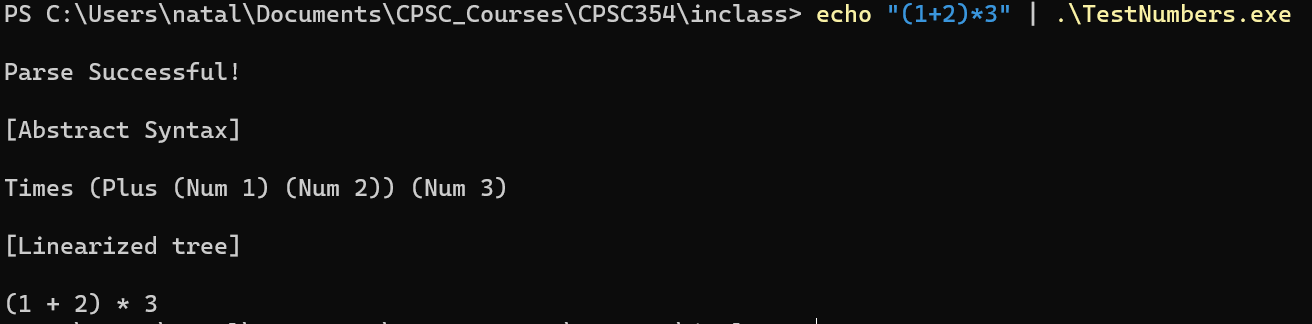
\includegraphics[width=15cm]{bnfc_exercise1d.png}

  \textbf{5. 1 + 2 * 3 + 4 * 5 + 6}\\
  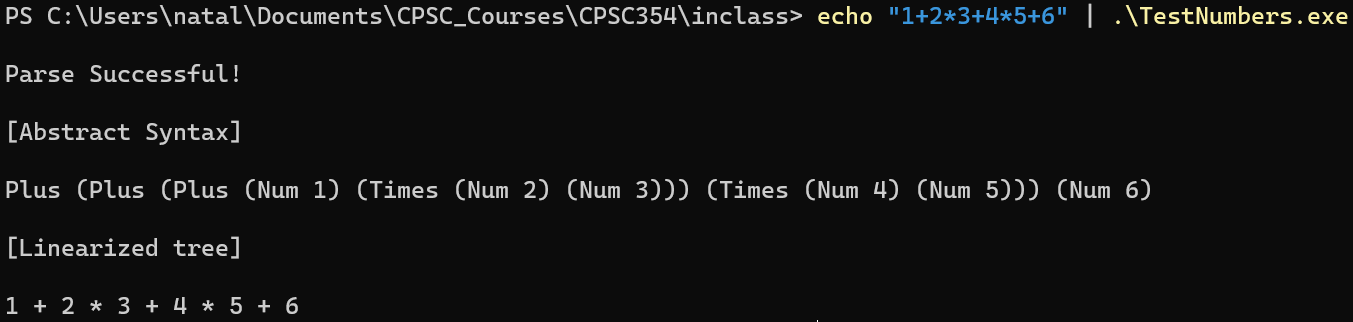
\includegraphics[width=15cm]{bnfc_exercise1e.png}
\end{center}


We can also look at the how the use of paranthesis affects the output. Here we will compare the output between 
\begin{center}
  \begin{itemize}
    \item[\ding{99}] 1. 1+2+3
    \item[\ding{99}] 2. (1+2)+3
    \item[\ding{99}] 3. 1+(2+3)
  \end{itemize}


  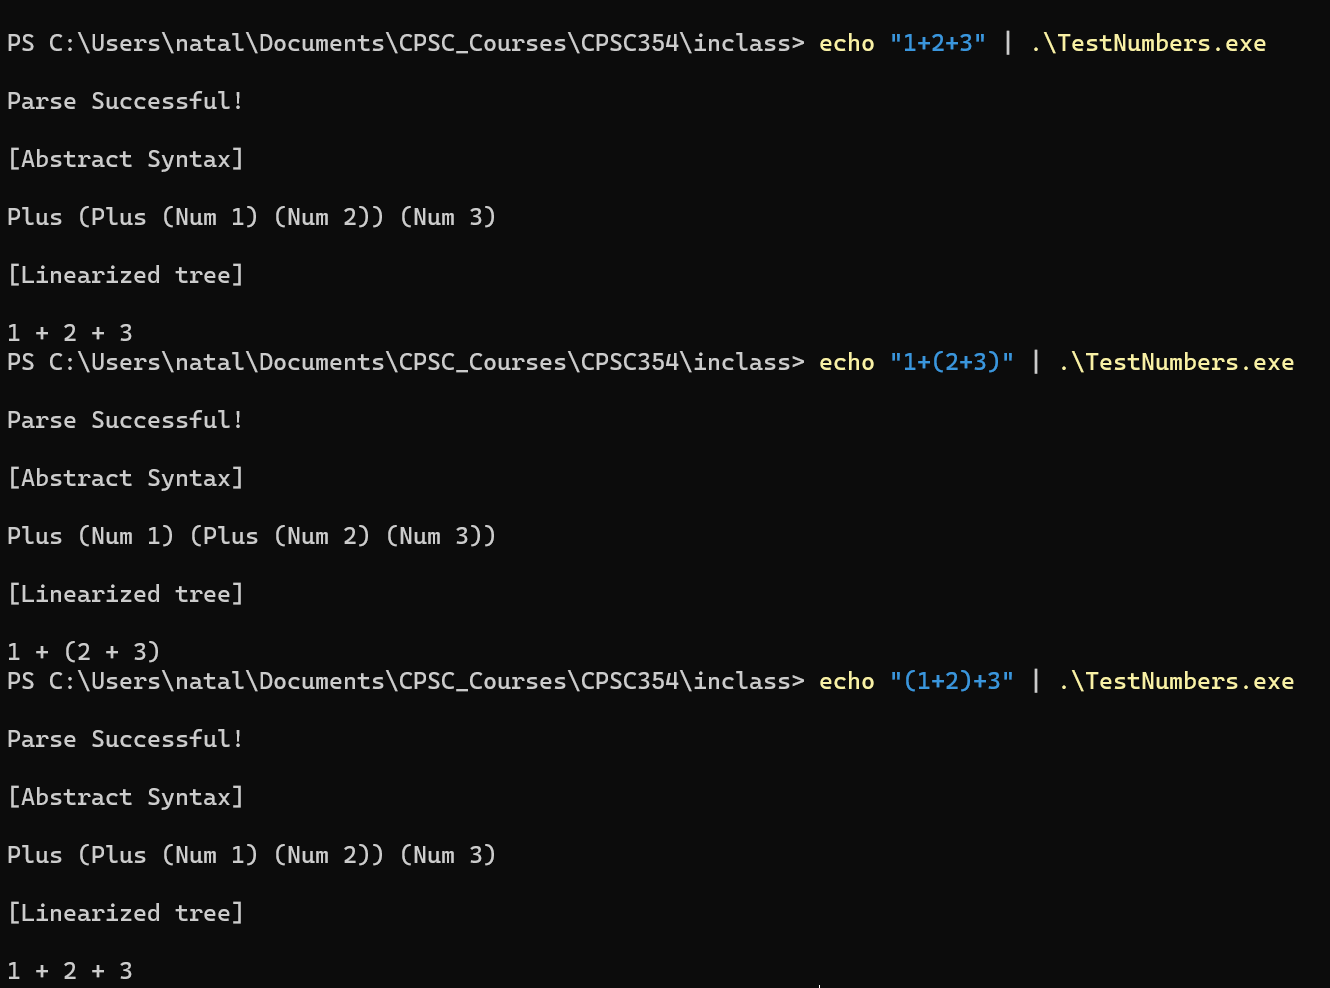
\includegraphics[width=15cm]{bnfc_exercise1f.png}
\end{center}
As you can see, the abstract syntax outputted differs depending on where or if the paranthesis are placed in the expression. The first and last output do yield the same result, implying 
that if the parser is not given any paranthesis, it will prioritize executing from left to right. In this case, the 1 and the 2 are added together first. Therefore, when the 2 and the 3 are 
placed in paranthesis, the abstract syntax changes as the order in which the addition functions are executed also changes. Overall, this homework focused on practicing the use of and establishing the BNFC 
environment as well as understanding how to convert concrete syntax into abstract syntax. \\

\subsection{Week 4}
This week's homework builds upon the previous assignment and focuses on understanding lambda calculus. Using the layout of the previous interpreter for addition and multiplication, I first had to 
modify the definitions and interpreter to read lambda calculus. The first step of the homework was to``use bnfc and the grammar of lambda-calculus [given] to create a parser for lambda-calculus expressions." 
I include the definition provided below: \\
\noindent
{\color{gray} \rule{\linewidth}{0.05mm}}
\begin{minted}{haskell}
  Abs.   Exp ::= "\\" Ident "." Exp ;  
  App.   Exp ::= Exp Exp1 ; 
  Var.   Exp1 ::= Ident ;

  coercions Exp 1 ;
\end{minted}
\noindent
{\color{gray} \rule{\linewidth}{0.05mm}}


Having generating a parser succesfully, I will now move on to the next section. Here, we will use the bnfc parser to write out the abstract syntax trees (in 2-dimensional notation) for 8 expressions. The first photo 
shows the 2-dimensional trees and the second code section shows the generated linearized abstract syntax tree I got from the bnfc-generated parser: 
\begin{center}
  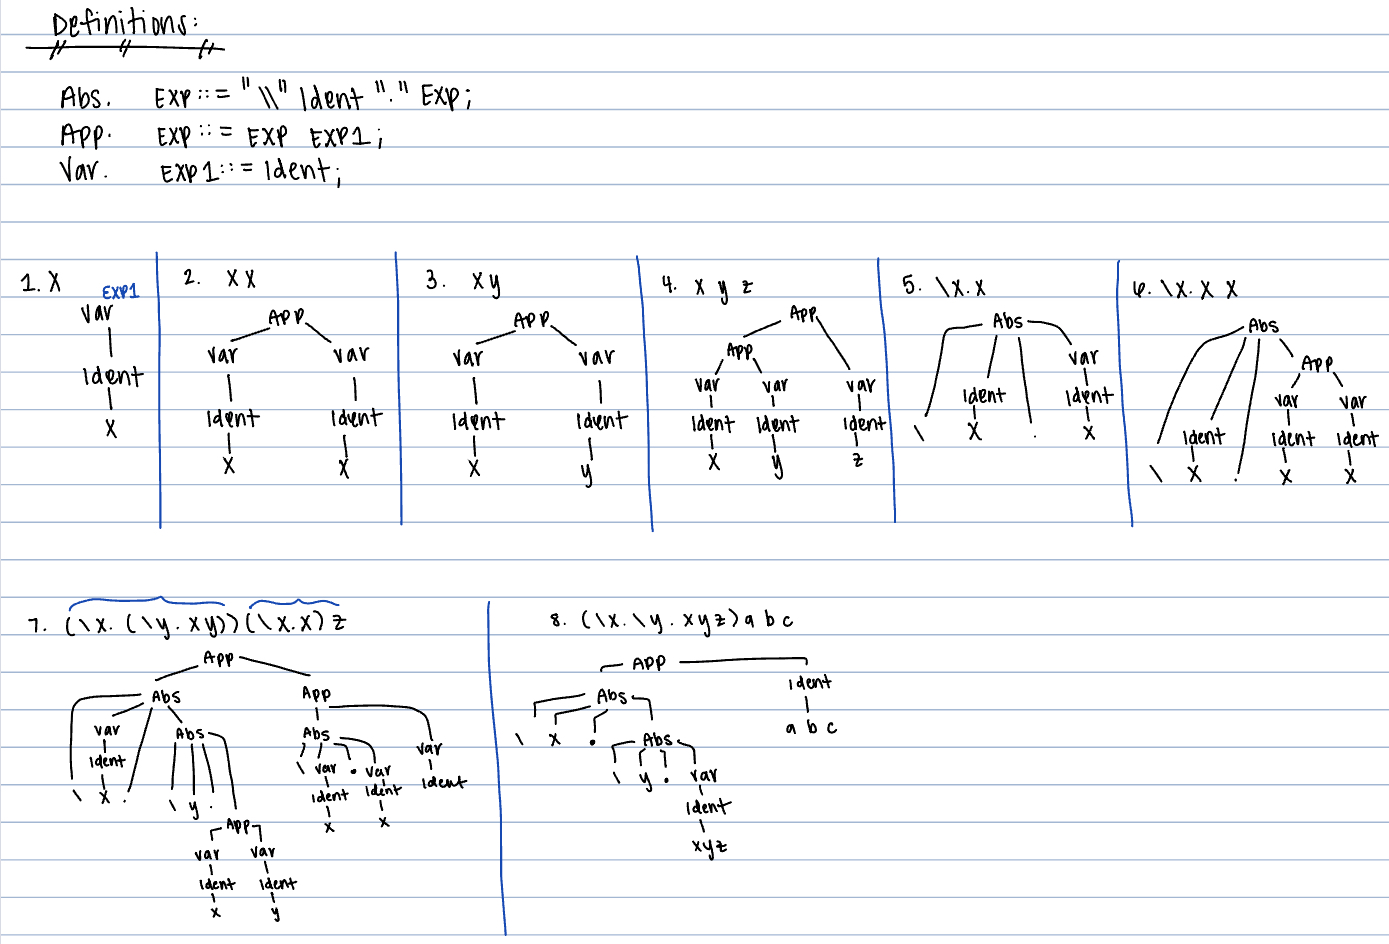
\includegraphics[width=15cm]{Week4hw_Trees.jpg}

  \noindent
  {\color{gray} \rule{\linewidth}{0.05mm}}

  \begin{minted}{haskell}
    x linearized: x
    x x linearized: x x
    x y linearized: x y
    x y z linearized: x y z
    \ x.x linearized: \ x . x
    \ x.x x linearized: \ x . x x
    (\ x . (\ y . x y)) (\ x.x) z linearized: \ x . \ y . x y (\ x . x) z
    (\ x . \ y . x y z) a b c linearized: \ x . \ y . x y z a b c
  \end{minted}

  \noindent
  {\color{gray} \rule{\linewidth}{0.05mm}}
\end{center}

As the final part of the homework, I finish the workout we began in class. This workout is a pen and paper computation based on the same definitions we described above. You should be able to see each step I took and my notes in green that help break 
up some of the notation, as it can get confusing quite quickly as the expression keeps expanding.
\begin{center}
  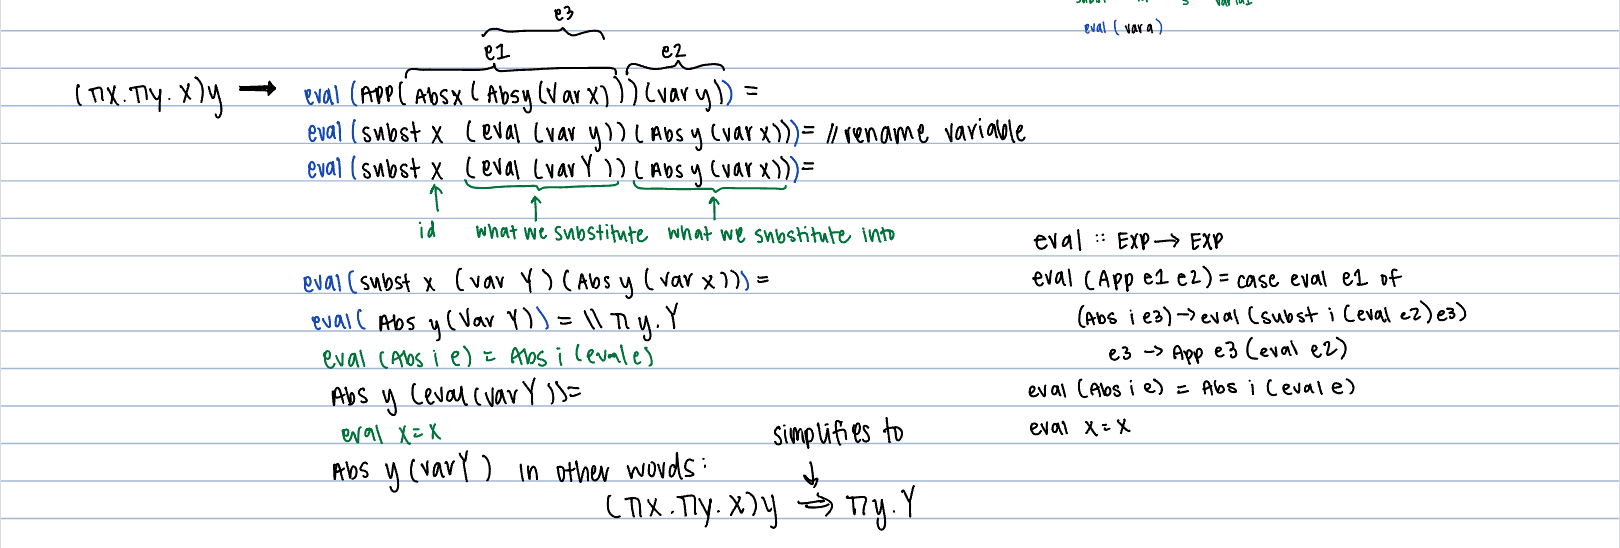
\includegraphics[width=15cm]{Week4hw_InClassProblem.jpg}
\end{center}

\subsection{Week 5}
\indent For this week's homework we will review two main topics. The first is our discussion of variables, bindings, scope, and substition and the second is our practice of understanding the interpretation of lambda calculus. 
Before I include the excercises for the section, I will include a review of the terminology and concepts we discussed. To start, there are three types of variables we introduced; they are as follows:
\begin{itemize}
  \item[\ding{99}] fresh variable - a variables that has not been used before 
  \item[\ding{99}] bound variable - a variables that can be renamed by a fresh variable without changing the meaning
  \item[\ding{99}] free variable - a variable that is not bound and receives its meaning from the context in which it appears 
\end{itemize}
\indent For example, in the expression \mintinline{haskell}{\x.x+y} the x is a bound variable and the y is a free variable. When we look at the scope of a variable, this simply means we have to take account the binding and paranthesis 
that apply to said variable. It's placement in the expression will affect the scope of the variable and therefore the meaning of it. As we can see, the \mintinline{haskell}{x} is bound by the \mintinline{haskell}{\x} in the equation and the y is simply a symbol. We do not have enough information 
to know what y is, so it serves as more of a placeholder and therefore is called a free variable. This is a common topic in programming, especially as we turn to look at functions, classes, 
and their respective variables. As a simple example, take the following function. \\
\noindent
  {\color{gray} \rule{\linewidth}{0.05mm}}
\begin{center} 
  \begin{minted}{javascript}
      var f = function(a) {
        return a+3;     
    }
  \end{minted}
\end{center}
\noindent
  {\color{gray} \rule{\linewidth}{0.05mm}}
\indent In the function defined above, the variable \mybluecode{a} only exists within the brackets of the function. Therefore, that is the scope of \mybluecode{a}. If \mybluecode{a} is referenced outside of its scope, an error will occur. Similarly, we can look at lambda calculus variables 
in the same way. \\ \indent The last term I will review is substitution. Substition is a common practice in mathematics, but it is important in lambda calculus as we begin to introduce the topic of capture avoiding substition or CAS. The reason we use CAS is to
prevent combining variables that may appear to be the same, but are not necessary equal. Therefore, the substition we will perform will avoid the ``capture" of these variables. Essentially, the idea is to look at the scope of the variables in the 
current expression and assess whether it is necessary to replace some of them with a fresh variable in order to dsitinguish the difference between itself and other variables in the following calculations. To see this in practice, I include the 
exercise provided for the homework below. \\

\noindent
  {\color{gray} \rule{\linewidth}{0.05mm}}
\textbf{Definition: } The function 
\begin{center}
  $f \circ g$
\end{center}
(pronounced "f after g") is the function obtained from taking the output of $g$ as the input of $f$. In the example, we want to replace the $x$ in $f(x) = x + y$ by 
$g(y) = y * 2$. It is tempting to write
\begin{center}
  $f \circ g(y) = f(g(y)) = 2 * y + y = 3y$
\end{center}
\noindent
  {\color{gray} \rule{\linewidth}{0.05mm}}
but this gives the \textbf{wrong} formula for $f \circ g$. Such mistakes arise from not taking proper care of the distinction of free and bound variables. I will consider the following three notes while addressing why this answer is incorrect. 
\begin{enumerate}
  \item What is the correct formula for the function $f \circ g$ in the example above?
  \item Use the notions of free and bound variables and score to explain your answer.
  \item Using lambda calculus write down a general formula for $f \circ g$ that works for abritrary f and g.
\end {enumerate}

Given what I have reviewed above, we can identify there is an issue in the above calculation regarding the variable $y$ and its scope. Although the $y$ variable in the functions $f(x)$ and $g(y)$ would be acceptable in many mathematical scenarios, this is 
not necessarily the case for us. Given that $y$ is a free variable in the function $f(x)$ and a bound variable in the function $g(y)$, we do not have enough information to ensure that they refer to the same value. It is possible that each $y$ is in fact a symbol referring to 
a unique value. In other words, the binding to $y$ is not in the scope of the instance $y$ in the function $f(x)$. Therefore, we cannot assume that it is bound to the same value. So, it is incorrect to simplify the expresion to $3y$. In order to correct this formula, 
we must use capture avoiding substitution. We can assign the $y$ in $f(x)$ a fresh variable to distinguish it from any other instances of $y$. The correct formula would therefore be: \\

\noindent
  {\color{gray} \rule{\linewidth}{0.05mm}}
\begin{center}
  $f(x) = x + Y$\\
  $g(y) = y * 2$

  \begin{align*}
    f \circ g(y) & = f(g(y)) \\
                & = 2 * y + Y \\
                & = 2y + Y
  \end{align*}
\end{center}
\noindent
  {\color{gray} \rule{\linewidth}{0.05mm}}

Since the $Y$ is a free variable it will remain in the solution as a symbol. Meanwhile the bound $y$ will be substituted with a value if one is provided. As a general formula for $f \circ g$, we can represent it as: 

\begin{center}
  $f \circ g(y) = $ \mintinline{haskell}{\y.f(g(y))}
\end{center} 

As you can see, we do not include the $x$ variable in this formula because it is being replaced by the output of $g(y)$. If we assign a value to $f \circ g$ we will only have to pass in one value, that of $y$, so we do not need it in the formula. \\



Now, for the second half of this homework, we will switch into the discussion of the lambda calculator interpreter we have been using and gaining a deeper understanding into how and when the rules apply. This will also give us a better understanding of the topics we already 
mentioned such as variables, bindings, scope, and substitution. We were given the following task:\\

To understand how the interpreter works do the following:
\begin{itemize}
  \item[\ding{99}] Use Interpreter.hs to evaluate in the style above (equational reasoning as in Example 1 and 2)  
  \begin{center}\mintinline{haskell}{(\x.\y.x)y}\end{center} 
  \item[\ding{99}]Follow the implementation of eval and subst line by line, but choose your own fresh names to simplify the computation.
  \item[\ding{99}] For each variable appearing in subst say what its binder is and what the scope of the binder is.
\end{itemize}

Below I will include three pictures. The first is a simple screenshot of the Interpreter.hs file in order to understand what lines I am referring to in my computation. The second picture is a screenshot of the terminal output when the interpreter file is run with the input of the function above. 
The third picture is my handwritten computation of the equation \mintinline{haskell}{(\x.\y.x)y}. 
In my computation, the lines in grey represent my explanations or references to what is prompting the next step of computation. I also used different color parentheses to avoid any misunderstanding of scopes of variables. Overall, the computation is quite simple. 
We must first evaluate the expression e1, which results in a recursive evaluation of both Abs cases in the expression. Once we have evaluated this, we can go back to the original expression and replace e1 for its evaluated value. Then, we can look at the definition of 
how to evaluation an App expression. This leads us to a substition. The reason this substitution is important is due to the fact that both $y$'s in the original expression are not necessarily equal in value. We must substitute one of them to avoid combining them. In this example, 
we substitute the \mintinline{haskell}{\y} for a reason. If we prioritize substitution this variable, we can easily replace the instances of $y$ it is binding. In this case, there are no $y$'s to replace in the body of the \mintinline{haskell}{\y.x} expression. Therefore, our 
result to this expression is \mintinline{haskell}{\A.y}. Since there are no $A$'s in the body of this, the expression would simply evaluate to \mintinline{haskell}{y}.

\begin{samepage}
  \begin{center}
    \textbf{Interpreter.hs}\\
    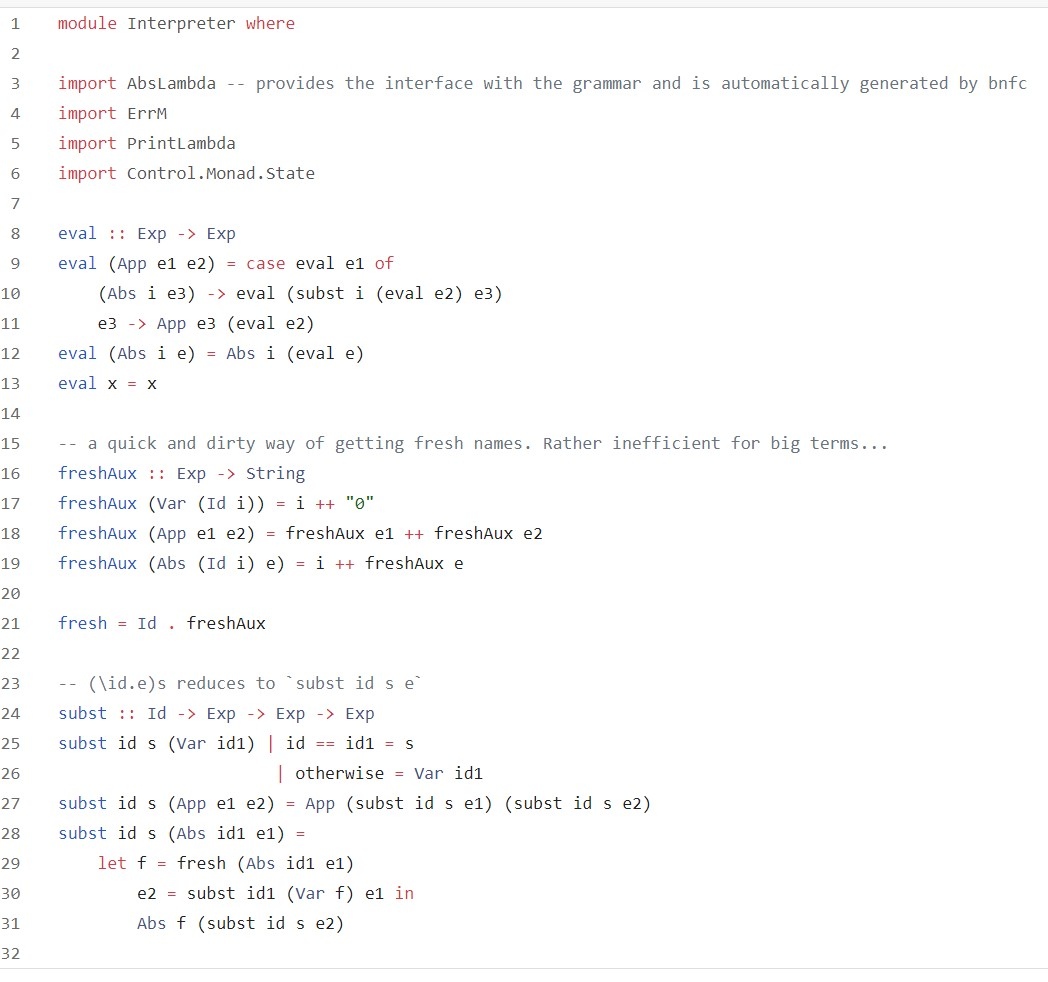
\includegraphics[width=13cm]{Week5hw_Interpreter.jpg}\\
  \end{center}
\end{samepage}

\begin{samepage}
  \begin{center}
    \textbf{Terminal Output}
    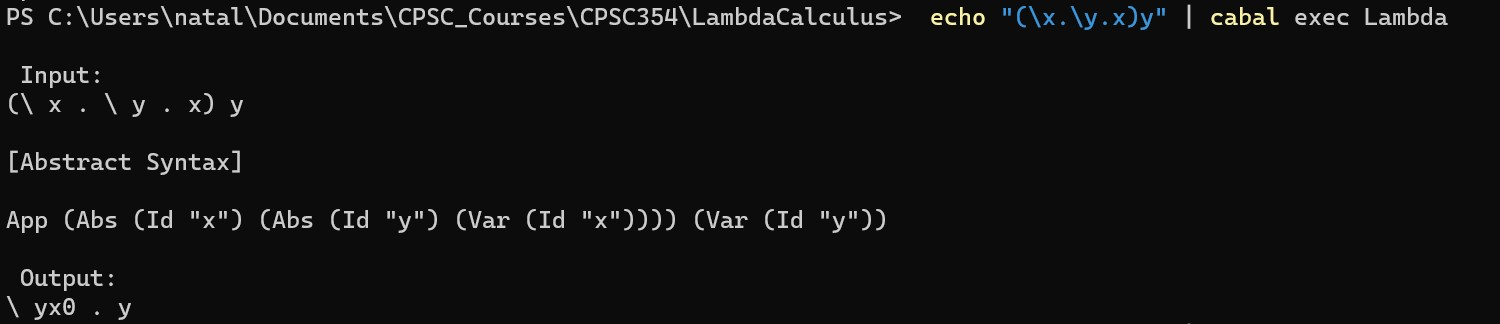
\includegraphics[width=15cm]{Week5hw_interpreterOutput.jpg}\\
  \end{center}
\end{samepage}

\begin{samepage}
  \begin{center}
    \textbf{Handwritten Computation}
    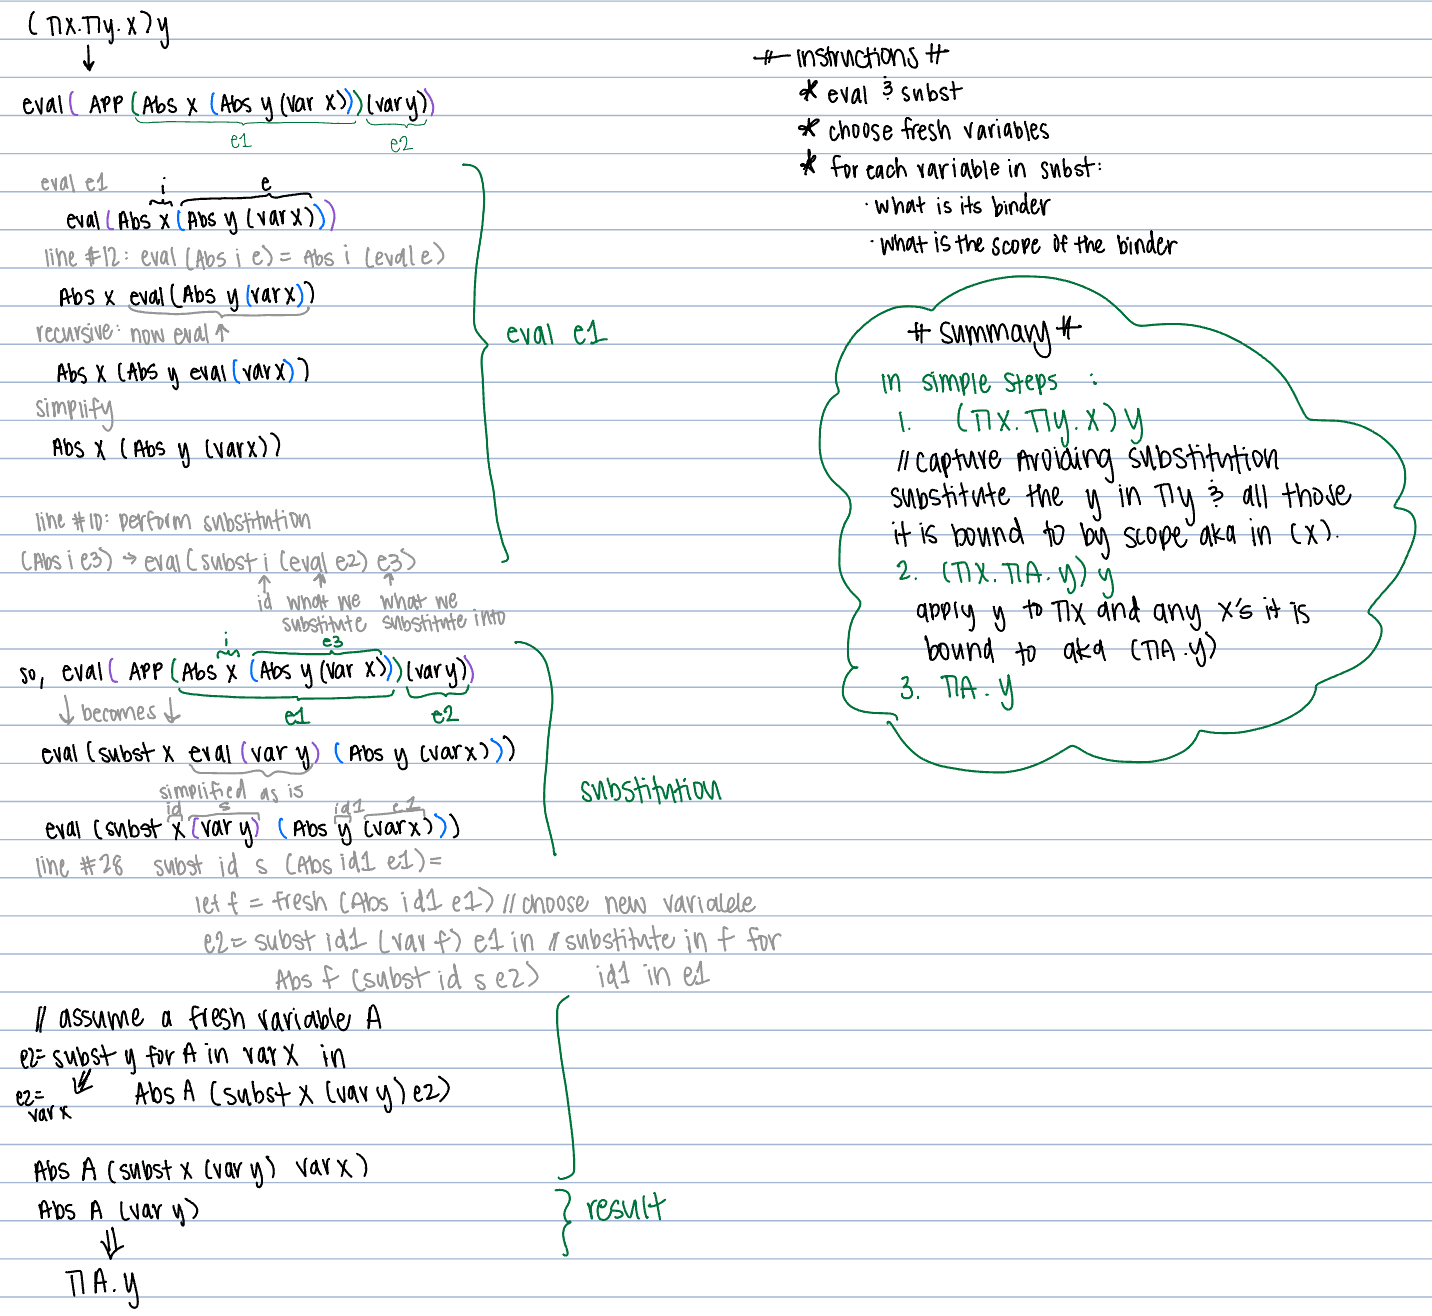
\includegraphics[width=15cm]{Week5hw_handwrittenInterpreter.jpg}
  \end{center}
\end{samepage}

\subsection{Week 6}

The aim of this week's homework is to review what we learned in class about ARSs. An ARS, or an Abstraction Reduction System, provides you with rules that will allow you to reduce any expression composed of the letters in the given alphabet. I will first include the example we 
did in class and then include the excercises given to us as practice. 

So, the in-class example is as follows. Given the rewrite rules below, answer these questions: \\
\noindent
  {\color{gray} \rule{\linewidth}{0.05mm}}
\begin{center}
  \begin{minted}{haskell}
    aa -> a 
    bb -> a 
    ab -> b
    ba -> b 
  \end{minted}
\end{center}
\noindent
  {\color{gray} \rule{\linewidth}{0.05mm}}

\begin{itemize}
  \item[\ding{99}] \textbf{Why does the ARS terminate?}
    \begin{enumerate} 
      \item[] This ARS terminates when there is only one character left in the expression because this means there are no more rules that will shorten the string. 
      In other words, none of the given rewrite rules can be applied. Following this logic, there are three final outcomes that an expression can be simplified to. 
      These are \mintinline{haskell}{a}, \mintinline{haskell}{b}, and \mintinline{haskell}{e}. (Note: \mintinline{haskell}{e} stands for epsilon, which represents the empty string). The ARS cannot apply any of these rules to a single character or no character 
      because each rule begins with a pair of letters. Each string will simplify to a single character because the rules account for every possible combiantion of \mintinline{haskell}{a} and \mintinline{haskell}{b}. 
    \end{enumerate}
  \item[\ding{99}] \textbf{What are the normal forms?} 
    \begin{enumerate} 
      \item[] The normal forms, or the strings that you cannot rewrite, are \mintinline{haskell}{a}, \mintinline{haskell}{b}, and \mintinline{haskell}{e}.
    \end{enumerate}
  \item[\ding{99}] \textbf{Is there a string \mintinline{haskell}{s} that reduces to both \mintinline{haskell}{a} and \mintinline{haskell}{b}?}
    \begin{enumerate} 
      \item[] There is not a string that reduces to both a and b. 
    \end{enumerate}
  \item[\ding{99}] \textbf{Show that the ARS is confluent.}
    \begin{enumerate} 
      \item[] An ARS is confluent if ever``peak" contains a``valley". To test this, we will take the five cases of overlapping pairs, or the critical pairs, and compute whether these 
      two expressions will converge. In the picture below, you can see how I tested these cases. The reason we want these to converge is because we want to see if they will all possible 
      routes will simplify to the same end result. So, we take each possible overlap and draw out the routes one could take to simplify it. In these cases, the left arrow points to the 
      string that results from applying the appropriate rewrite rule to the left-most pair of letters in the original string and copying over the last letter. The right arrow points to
      the string that reults from copying over the first letter and applying the appropriate rewrite rule to the right-most pair of letters. We can see that in every case, the different 
      routes of computation converge to the same end string. Therefore, we can say that this ARS is confluent. \\
      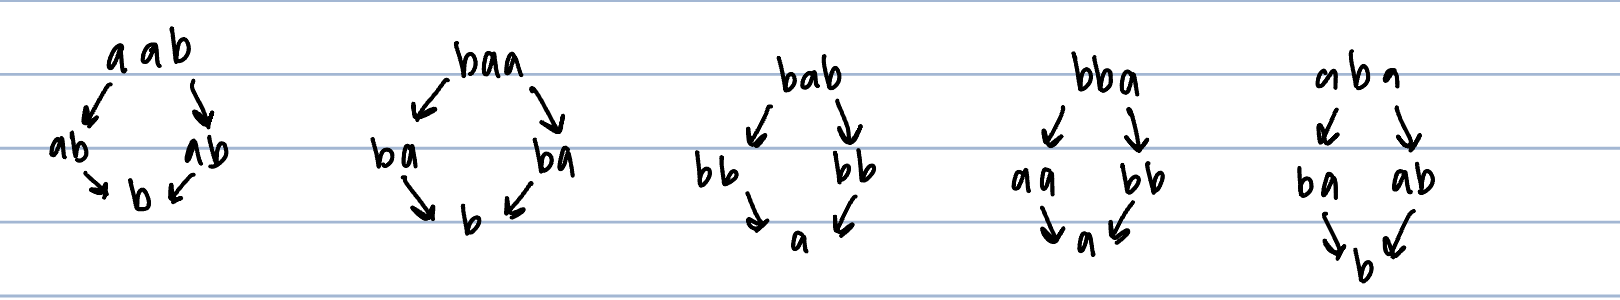
\includegraphics[width=15cm]{confluent.png}\\
    \end{enumerate}
  \item[\ding{99}] \textbf{Replacing \mintinline{haskell}{->} by \mintinline{haskell}{=}, which words become equal?}
    \begin{enumerate} 
      \item[] If we replace \mintinline{haskell}{->} by \mintinline{haskell}{=}, then all words that simply to \mintinline{haskell}{a} become equal and all words that simplify to 
      \mintinline{haskell}{b} become equal. Logically, this makes sense because if two strings simplify to the same letter, then the rewrite rules can be used backwards to result in either 
      of the original strings. As we discussed this question and as I tested many cases to understand the nature of the rules, we also discovered that if a string contains an odd number of \mintinline{haskell}{b}s its 
      normal form is \mintinline{haskell}{b} and if a string contains an even number of \mintinline{haskell}{b}s then its normal form is \mintinline{haskell}{a}.
    \end{enumerate}
\end{itemize}


Now having reviewed the in-class example, we will look at the assigned exercises. First, we are prompted to draw a picture for each of the following ARSs:

\noindent
  {\color{gray} \rule{\linewidth}{0.05mm}}
\begin{enumerate}
  \item[\ding{99}] \mintinline{haskell}{A = {}}
  \item[\ding{99}] \mintinline{haskell}{A = {a} , R = {}}
  \item[\ding{99}] \mintinline{haskell}{A = {a} , R = {(a,a)}}
  \item[\ding{99}] \mintinline{haskell}{A = {a, b, c} , R = {(a, b), (a, c)}}
  \item[\ding{99}] \mintinline{haskell}{A = {a, b} , R = {(a, a), (a, b)}}
  \item[\ding{99}] \mintinline{haskell}{A = {a, b, c} , R = {(a, b), (b, b), (a, c)}}
  \item[\ding{99}] \mintinline{haskell}{A = {a, b, c} , R = {(a, b), (b, b), (a, c), (c, c)}}
\end{enumerate}
\noindent
  {\color{gray} \rule{\linewidth}{0.05mm}}

\includegraphics[width=20cm]{arsDrawn.png}

Lastly, we will find an example ARS for each of the following combinations in the table. I include my solution as a screenshot from my digital handwritten notes. 
\begin{center}
  \begin{tabular}{||c c c ||} 
   \hline
   confluent & terminating & unique normal forms \\ [0.5ex] 
   \hline\hline
   true & true & true \\ 
   \hline
   true & true & false \\
   \hline
   true & false & true \\
   \hline
   true & false & false \\
   \hline
   false & true & true \\
   \hline
   false & true & false \\
   \hline
   false & false & true \\
   \hline
   false & false & false \\ [1ex] 
   \hline
  \end{tabular}
\end{center}
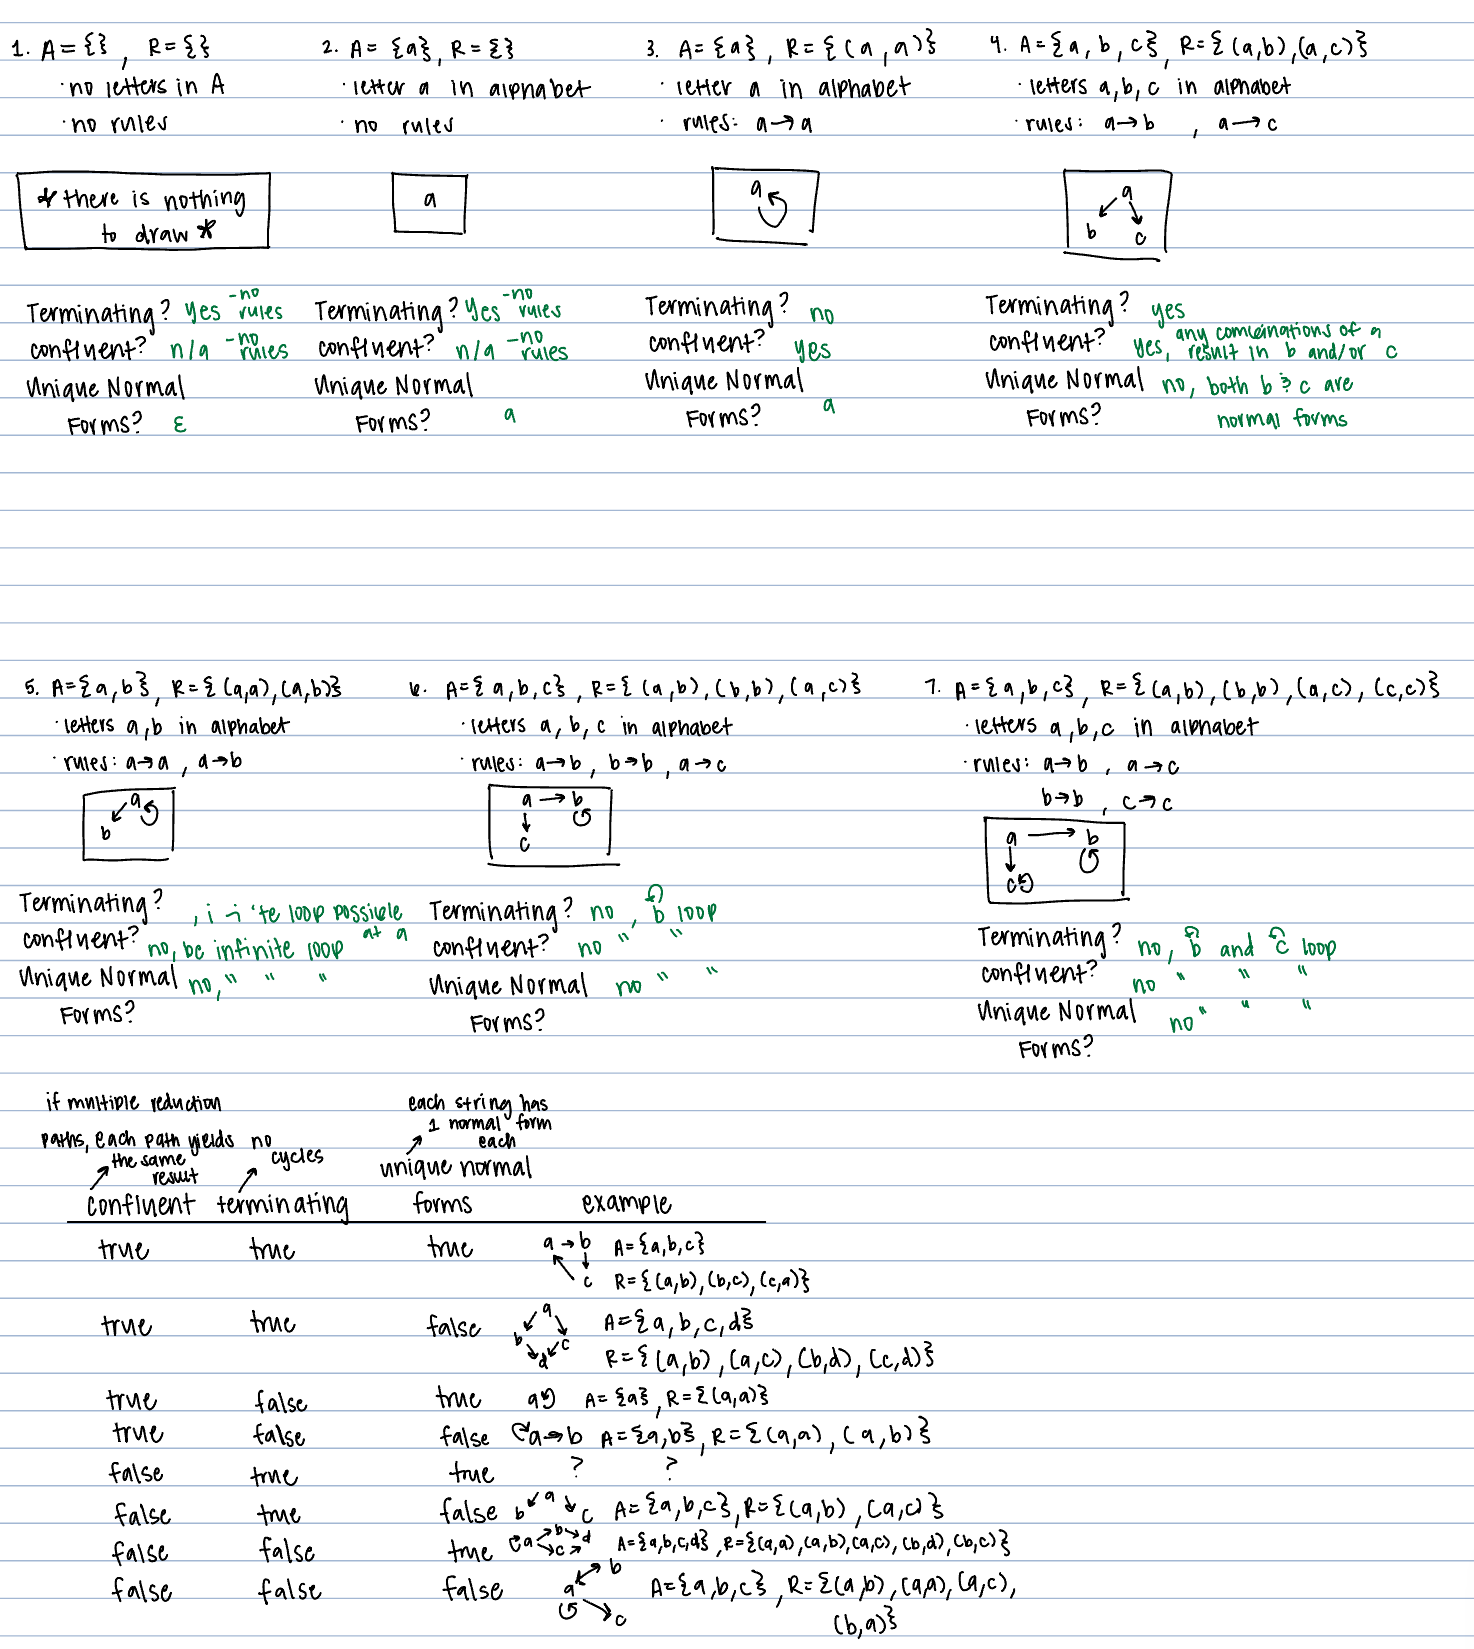
\includegraphics[width=15cm]{arsTable.png}

\textit{EDIT:} I add this note after having gone over a few of the examples above during our lecture. One of the main ideas we discussed was whether we could say that any of the three properties (that is: confluence, termination, and unique normal forms[UNF]) 
implies the others. We were ultimately able to agree upon the idea that if an ARS is both confluent and terminating then this implies it has UNFs. The confluence gives the ARS its uniqueness given that all ``peaks" have a ``valley" that lead it to the same 
end result. The termination of the ARS means it has normal forms. So, together they imply the existence of unique normal forms for the ARS. Having this new understading of the relationships of these three properties, we can look back at my notes and 
note that some of my examples are incorrect. Specifically, the row that describes an ARS that is confluent and terminating but does not have UNFs. This is not possible since the first two imply the last property. From my understanding
this would also mean that when either of the first two are false, the UNFs property must be false as well. I include an edited version of my notes below.

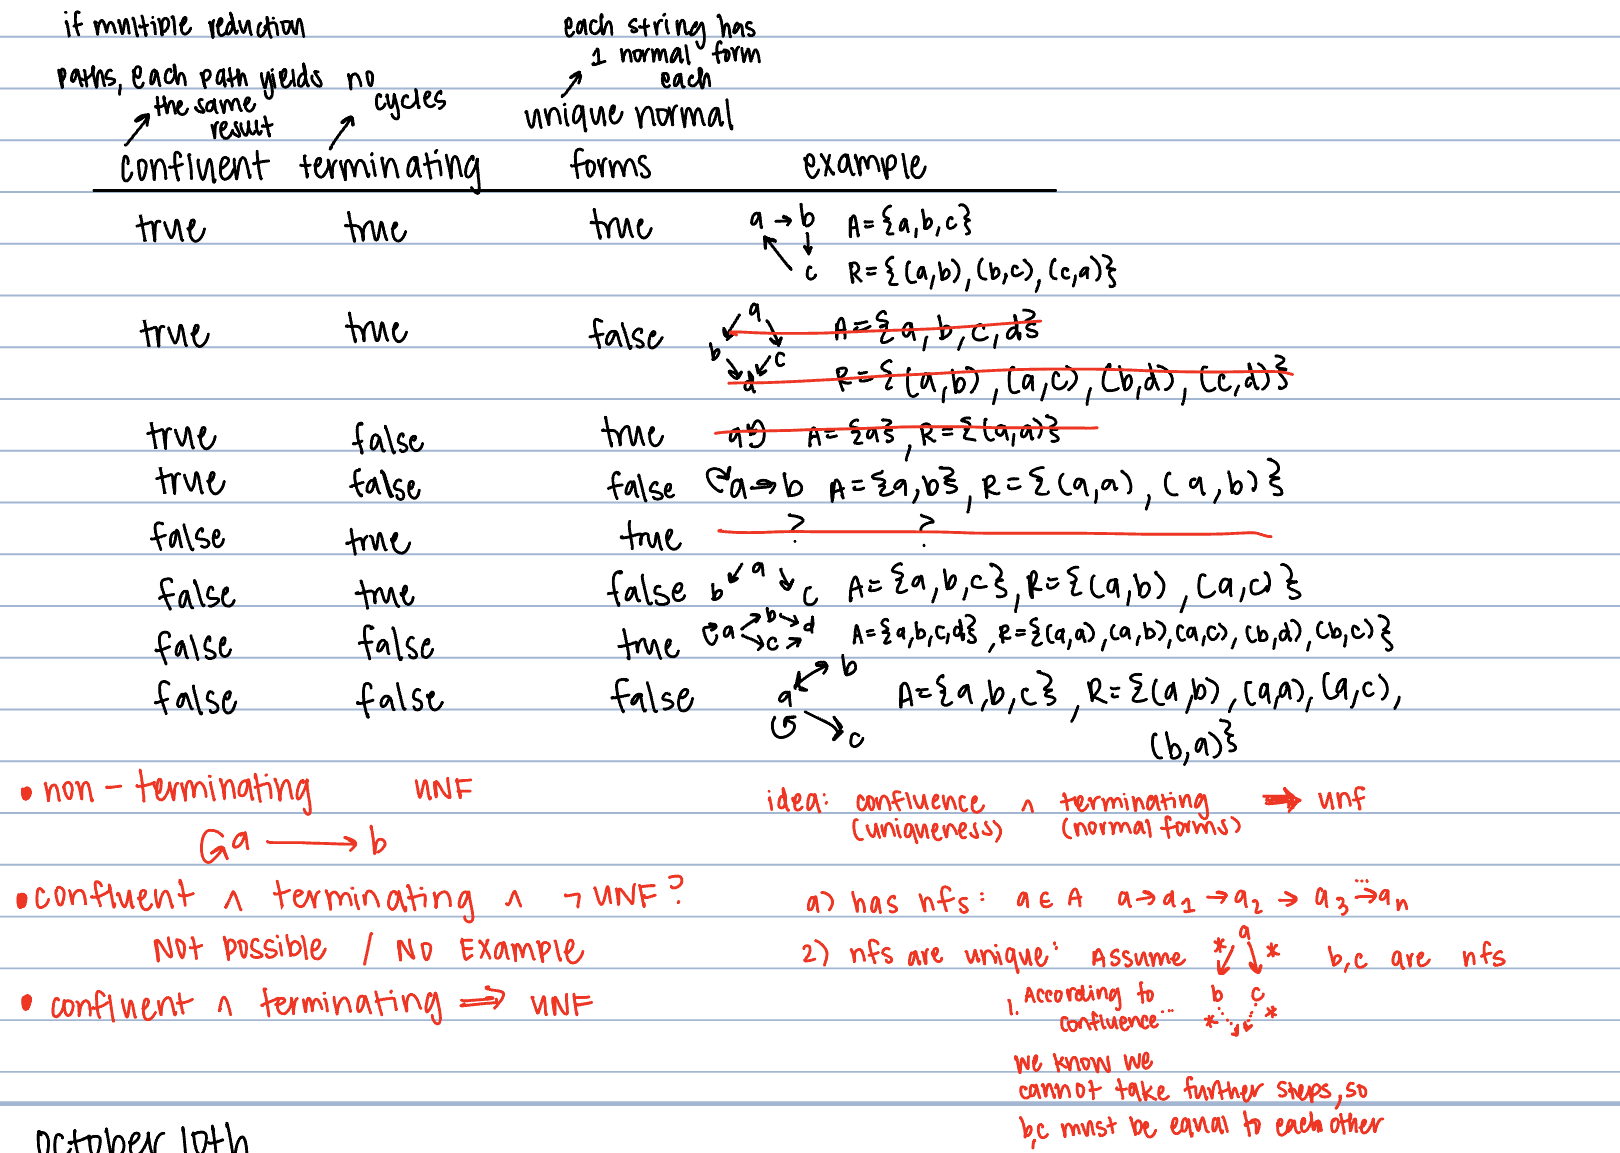
\includegraphics[width=15cm]{arsTableEdit.png}


\subsection{Week 7}

\indent For this week's homework we are reviewing what we learned about invariants. An invariant is a property we can identify that remains unchanged regardless of the input or the operations performed. An easy example for an invariant is to think of a mathematical 
formula that we commonly use. The area of a rectangle or the conversion from Fahrenheit to Celsius are two examples. Regardless of the measurements given to you, the formula of an area of a rectangle will always hold true and will not change. So, this relationship
or this formula is an invariant. Now, we can use invariants to prove or disprove scenarios. If we can prove that an invariant does not apply to a case, then that case should be false. \\

In class, we looked at the chessboard puzzle and used the invariant of how many white squares there were compared to black squares based on which tiles were removed. For this homework, I will look at one of the puzzles we did not discuss in class, but 
that was included as an example of a puzzle we could discuss, the Tetris Puzzle. I include the description of the puzzle in the below image. \\

  \begin{center}
    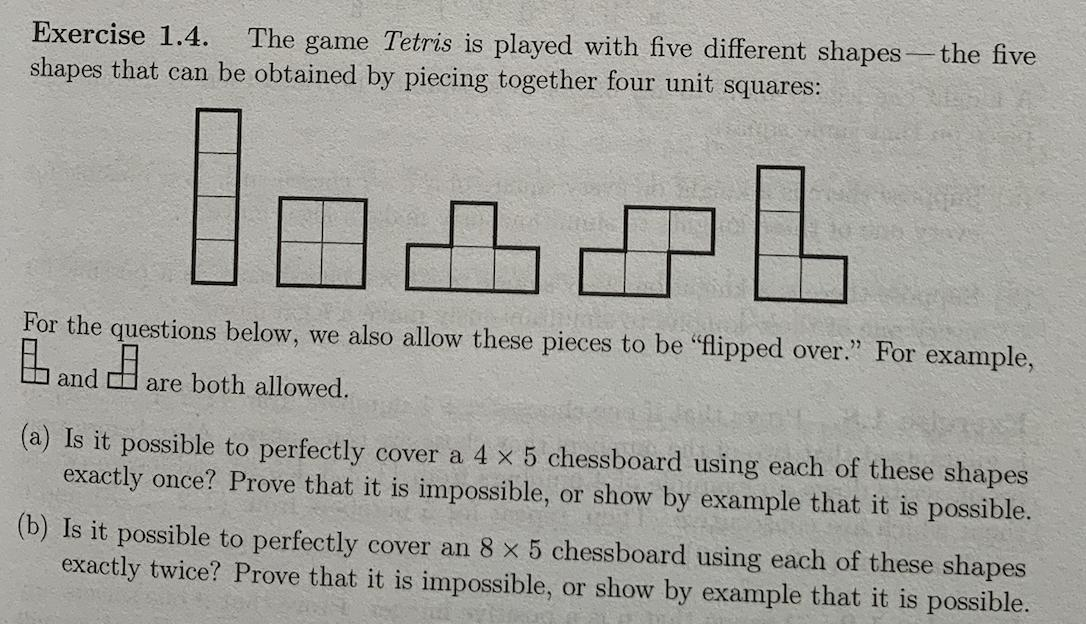
\includegraphics[width=15cm]{tetrisDesc.jpg}
  \end{center}

I stared at this problem for a while, trying to figure out a way to determine if I could fill the board with some sort of formula or invariant. After multiple failed attempts, I thought it was impossible to find a configuration that would successfully cover the 
4x5 board with the tetris tiles. The number of tiles of the five tetrinomes was equal to the number of tiles on the board, 20. However, they weren't fitting together in a way that would be acceptable. So, I looked back at our in-class example, the chessboard 
puzzle, and decided to use a similar approach. If we color the 4x5 grid with alternating colors, just like a chessboard, and the 5 tetrinomes as well, we can make an interesting observation. The board results in 20 total tiles, so 10 white tiles and 10 black tiles. 
The tetrinomes result in either 11 black tiles and 9 white tiles or 9 black tiles and 11 white tiles depending on where the alternations colors begin. In each case, the number of black and white tiles is not equal to the those on the 4x5 grid. If we look at it this way, 
we can reason that there is no possible configuration for the tetrinomes to cover the grid completely. The invariant here would that $the number of black tiles - the number of white tiles$ needs to equal zero. Here, this formula would equal $2$ or $-2$, not zero. I include 
my drawing of the tetrinomes and grid with alternating colors below. \\

  \begin{center}
    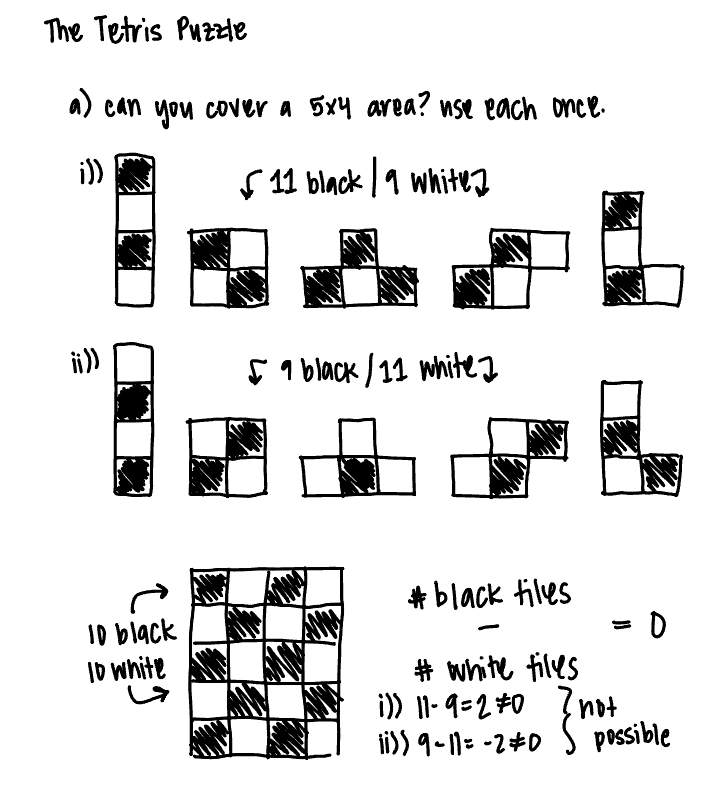
\includegraphics[width=9cm]{tetrisA.png}
  \end{center}


Now that we have discussed part a, part b is asking us if we can cover an 8x5 board by using each of the tetrinomes exactly twice. Let's use the same logic here. Again, the tiles and their colors remain the same and board simply expands. 
If we are using each tetrinome exactly twice, this means we have three possible combinations of colored tiles. The only tetrinome that affects this is the T shape so lets focus on this. We can have two T's with more black tiles each, two T's with more white tiles each, or 
two T's, one with more black tiles and the other with more white tiles. This leaves us with three possible combinations of total colored tiles. \\

\begin{itemize}
  \item[\ding{99}] 1. 22 black tiles, 18 white tiles 
  \item[\ding{99}] 2. 18 black tiles, 22 white tiles 
  \item[\ding{99}] 3. 20 black tiles, 20 white tiles
\end{itemize}

The first two cases, of course, indicate it is not possible to cover the 8x5 grid with those particular combinations of tiles because of the mismatch between the number of each colored tile on the grid and by the tetrinomes. However, the third case does match that of the grid, so we can say that there is a configuration that will allow us to cover the 8x5 grid with that 
combination of tiles. The two T tiles in thise scenario are opposite of one another, so their uneven number of alternating colors cancel out here. The invariant, again, here also proves this because $22-18$ and $18-22$ are not equal to zero but $20-20$ is equal to zero. Below, I include 
again my drawings of the tiles and the configuration I found to satisfy the puzzle using my knowledge of the invariant. \\

\begin{center}
  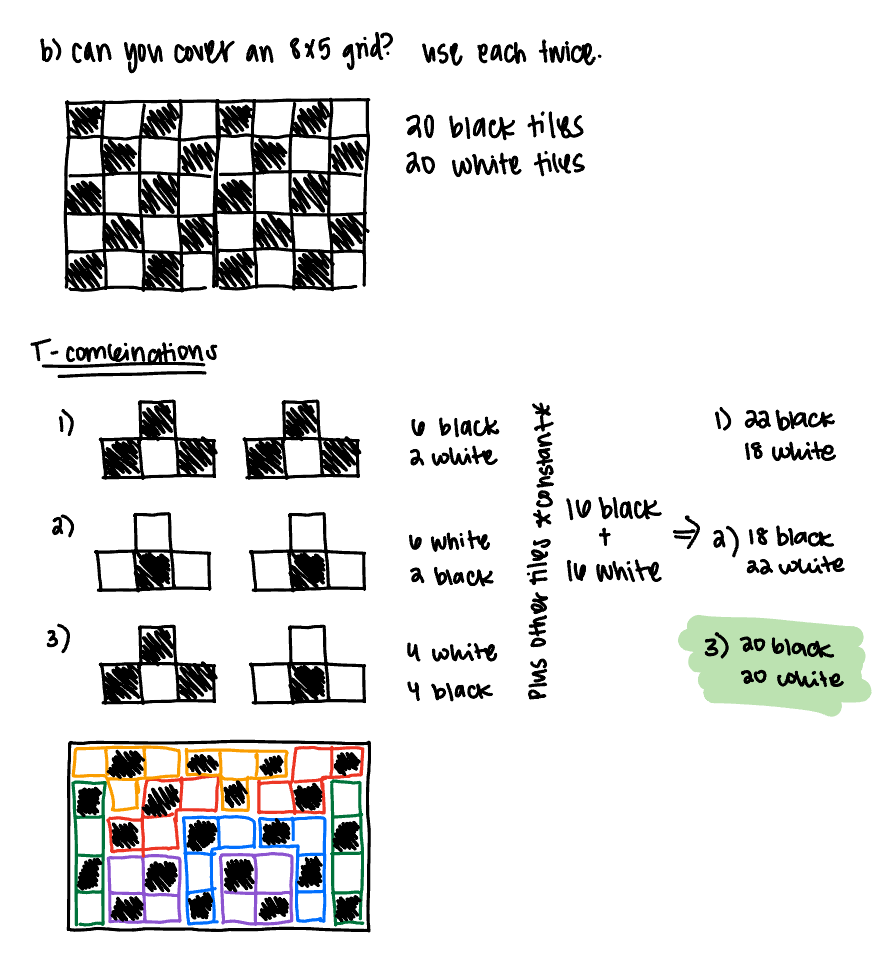
\includegraphics[width=10cm]{tetrisB.png}
\end{center}

By using invariants, we can go about proving or disproving questions more efficiently rather than trying to plug in values until we can find a set that is satisfactory or until we notice the pattern. It allows us to apply our mathematical foundations and definitions to other areas, 
such as computer science. 


\subsection{Week 10}

For Week 10's homework, we will look at what the Prisoner's Dilemma is and how we can use the Blockly project Prof. Kurz set up the understand it better as well as testing new strategies. The basic idea of the Prisoner's Dilemma is as follows. There are two prisoner's who are given the chance to either support the other or sell them out, in a sense. The payoff for each prisoner 
is dependent upon the combination of what both prisoner's decide to do. Given these different outcomes, each person must decide which option to choose in order to maximize their payoff. Below is an image describing the combinations possible and their effects on either prisoner. 

\begin{center}
  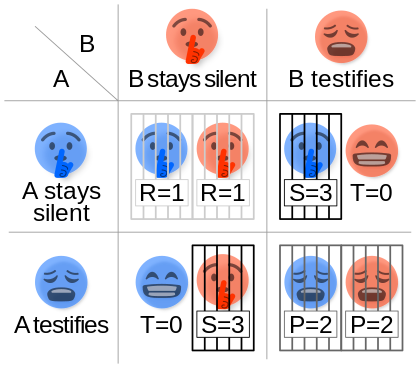
\includegraphics[width=10cm]{prisoner_dilemma_desc.png}
\end{center}

The blockly project we will be observing functions as a server-client model where we will have to open two browsers, one for each prisoner, and send our strategy for them to use for their decision-making. As an example, I include two screenshots of the blockly project functioning, one for each of the prisoners. \\

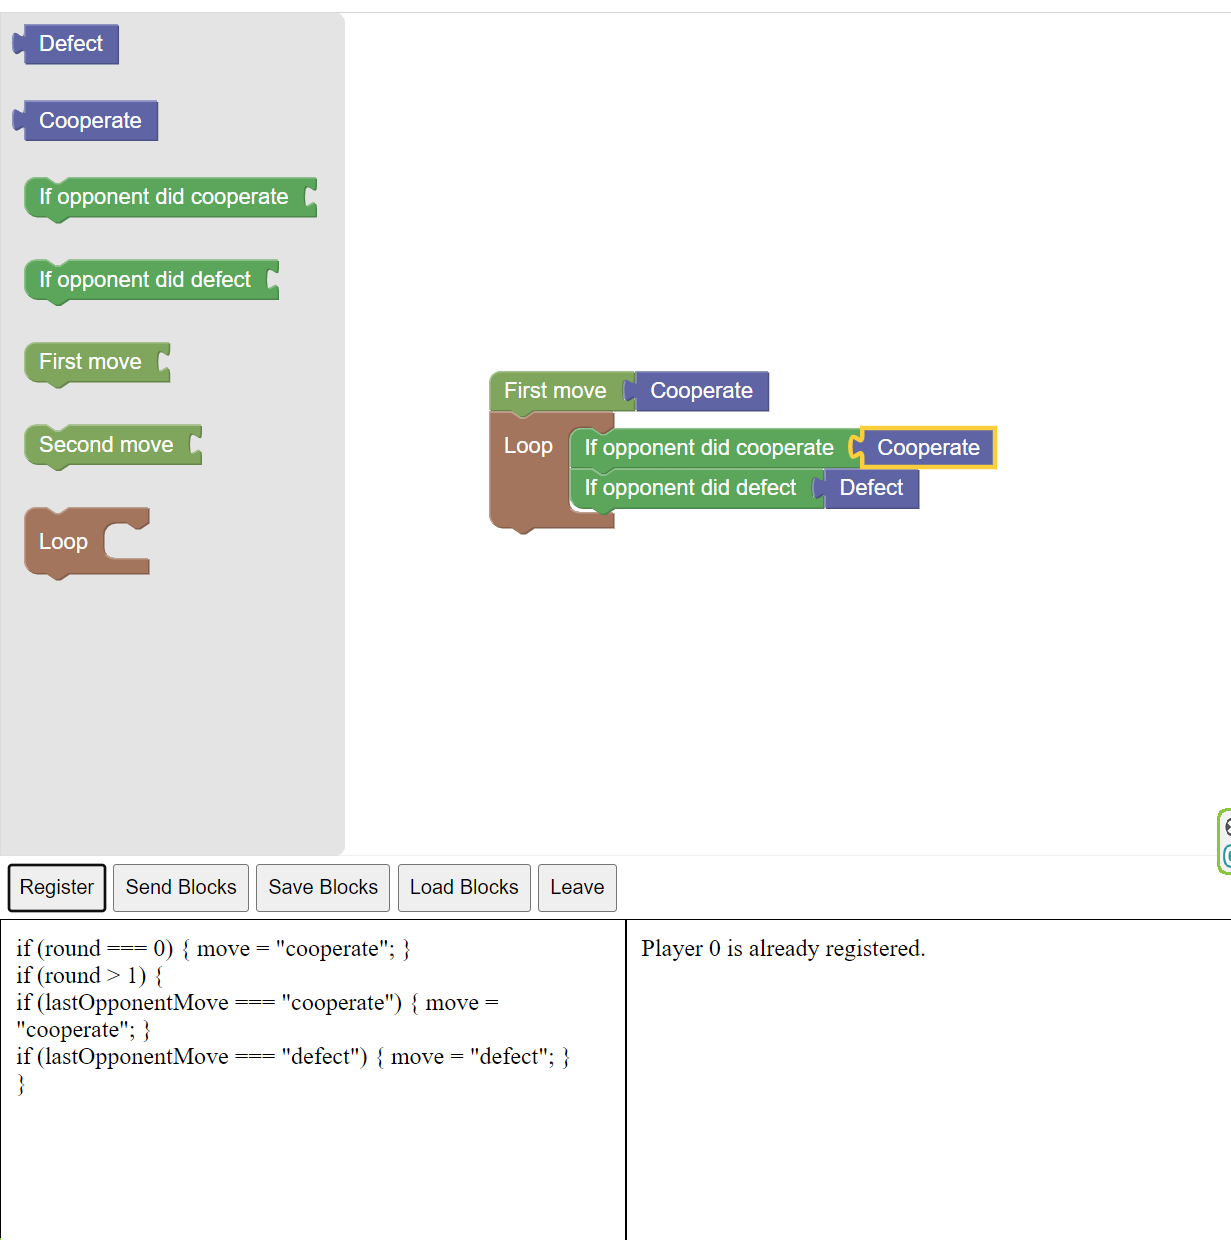
\includegraphics[width=8cm]{prisoner_blockly1.png}
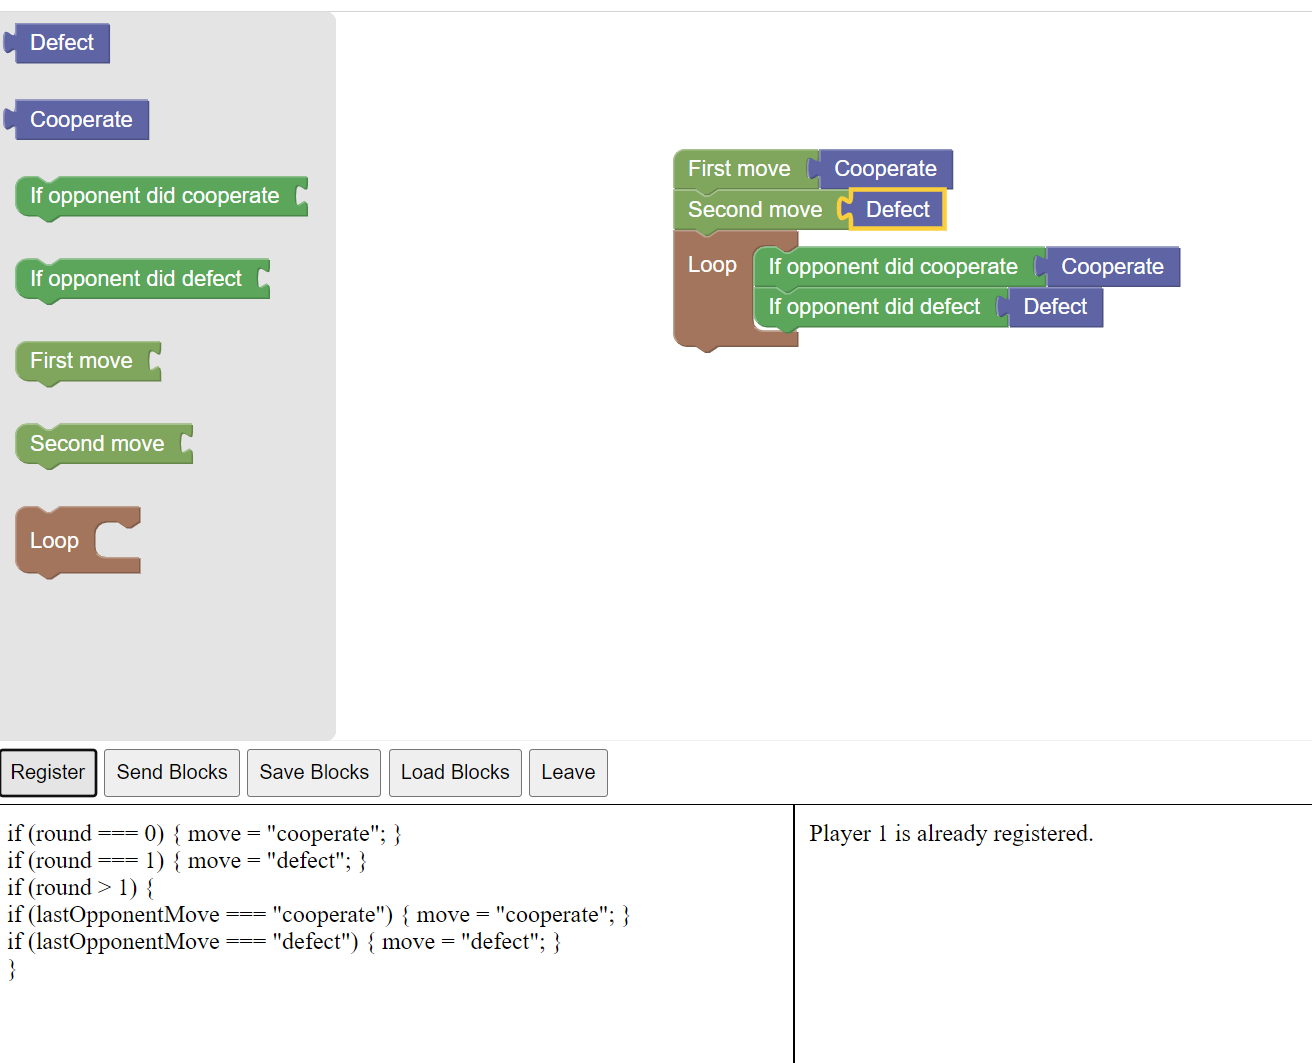
\includegraphics[width=8cm]{prisoner_blockly2.png}

Now that we have reviewed the Prisoner's Dilemma, we will answer the homework question below:
\begin{itemize}
  \item[\ding{99}] \textbf{When will one player be shown the result of the game? Explain why this happens and what part of the code implements this.}
\end{itemize}

When a player clicks on the “send blocks” button, this post request is executed. I will describe step-by-step what occurs based on my understanding using the debugger for this assignment. 

The server will first receive the request to execute the endpoint and receive both the player’s code and the player’s ID. It will then check if both players have submitted their code. If they have, the server will try to run the game using the \mintinline{javascript}{runGame(playerCodes[0], playerCodes[1])} function. 
The result of the game will then be sent to the client. If both players have not submitted their code, the server will wait for 10 seconds for the other player to respond with their code. At each second, it will check if the second player has submitted their code and the game has finished. If 
so, the game result will be sent to the client. If in the 10 seconds, there is no detection of the second player’s response, then the server will indicate it did not receive it. 

For both players to get the result of the game, both must submit their code relatively close to each other. In this case, it would need to be within 10 seconds of each other because that is how long the loop will keep checking for both responses. Otherwise, it is possible that only the second 
player gets the result. This is possible because the first player will stop checking for the second player’s code and will therefore not get the result of the game. The second player, however, when submitting its code will prompt the \mintinline{javascript}{runGame} function and then get the result once it completes. 
To fix this, I would consider changing the 10 second timeout on the loop checking for the second player’s code. Otherwise, this situation will continue to be possible. A snippet of the code I am referencing is included below. 

\noindent
{\color{gray} \rule{\linewidth}{0.05mm}}

\begin{minted}{javascript}
// Players ready, run game
if (playerCodes[0] && playerCodes[1]) {
        console.log("Both players have submitted their code. Running the game..."); // Log before running the game
        try {
            let { index, logs } = runGame(playerCodes[0], playerCodes[1]);
            gameIndex = index
            gameLogs = logs
            gameDone = true

            // Send the result back to the client (only this client's response)
            console.log("Execution result: ", { output: gameIndex, logs: gameLogs, payoff: gameLogic.env.payoff });
            res.status(200).send({ output: gameIndex, logs: gameLogs, payoff: gameLogic.env.payoff });
        } catch (error) {
            console.error("Error executing code: ", error.message);
            res.status(500).send({ error: error.message });
        }
        console.log("Finished processing /execute request");

        // Reset playerCodes
        playerCodes = {};
    } else {
        console.log("Waiting for the other player to submit their code."); // Log when waiting for the other player
        // Wait 10 seconds for other player response
        for (let i = 0; i < 10; i++) {
            await new Promise((res) => { setTimeout(res, 1000); }); // Wait 1 second
            console.log(`Checking if game done (${i})`)
            if (gameDone) {
                console.log('Game done! Sending game result to client')
                res.status(200).send({
                    message: 'Got other player response.',
                    output: gameIndex,
                    logs: gameLogs,
                    payoff: gameLogic.env.payoff
                });
                gameDone = false
                return;
            }
        }
        console.log('Game done not detected, returning to client')
        res.status(200).send({ message: `Did not receive other player code yet. Standing by` });
    }
\end{minted}

\noindent
{\color{gray} \rule{\linewidth}{0.05mm}}



This assignment also introduced me to how using a debugger is helpful because it allows you to step through the code and see the changes in variables and the flow of function calls line by line. I had some issues using the debugger in that it stopped working suddenly and I have not been able to find a solution yet, but I plan to keep 
testing it and trying to fix it so I can use it for future projects and assignments. I had heard of and known about debuggers before, but I had never actually tried to install one and use it for my code, so this was interesting to test out for me. I am curious as to if there are debuggers that could be applied to me game dev specific coding.
It is in the language C\#, but I wonder which debuggers are out there that can help solve Unity-specific errors. Additionally, I wnant to acknowledge my use AI for this assignment to understand the code a bit better, but all that was written above is my own work (as my reflections I mean). 


\section{Lessons From the Project}\label{Lessons From the Project}


\subsection{Project Description} 

As I mentioned in the introduction of this report, another huge part of coursework for this class in the semester-long group project. I would like to not only provide a better description of what this project was for my group but also talk about what that looked like for me 
personally and what some of the lessons I learned from the process were. My group wanted to create a project that was related to bridging the gap between the typical user and useful information about their health and nutrition. So, we decided to build a progam where a user could 
obtain nutritional information about their meals and exercise routines. In addition to being related to health, we also wanted to create something that was user-friendly and accessible to the everyday person, regardless of their coding background. In other words, anyone should be able 
to use our program and should not be deterred away in fear they might not have the knowledge to use it. \\

\subsection{Development Process} 

In order to achieve our goals for this project, we had to plan out how we were actually going to develop such a program. Although it happened to be a requirement for the class, the use of the Blockly API really helped our group be able to provide the user-friendliness of this program. Given 
that most people do not come from a coding or engineering background, it was important for us to make our program intuitive for users to interact with and using the Blockly API allowed us to do just this. Rather than users having to look at and try to write code themselves, which could 
very well deter many users from even trying out our program, our program allows them to connect blocks instead, which then generate code based on our implementation. This is particularly important because as we added in other components such as the API calls to the Nutritionix API, which I will 
explain later, and the need to set up a server. \\

I mentioned the Nutritionix API because this is also a key component in our project. Nutritionix maintains a database of both nutritional information of food and exercise activities and their API allows us to access this information. Nutritionix also has a natural language processing model that 
we take advantage of. For us, this means that rather than having to traverse the database ourselves and matching the user's input with posssible entries, we can use their model to complete this process for us. For those that are familiar with what an API is, we know that this can prove to be a very 
powerful tool. However, for those that do not, it can be very daunting to learn about and manage using API call endpoints. Not only would someone have to learn about APIs, but they would also have to learn how to implement it within their coding environment. The main takeaway here is that this can 
prove to be a barrier of entry for accessing such a useful database. The goal of our project is to break this barrier a little in order to allow users to access the API and it's benefits without having to deal with these challenges. \\


\subsection{Final Product}  

Now, reflecting back on our original goal for the semester, I can say that I do believe we made some good progress. However, as with any project, I still have some ideas and thoughts about how the project can progress and become better than what we have implemented so far. At this moment, we have 
the github pages site running successfully where a user can interact with the blocks in the toolbox and use them to administer API calls. A user can submit some text input and receive the results from the natural language processing model I mentioned. I think the main notes here for moving forward, both of 
which I will discuss in more detail in the Future Additions section, are that the user has to run the server themselves from their local computer and the output from the API can be somewhat hard to read. These are two of the biggest improvements I think can be made for this project. Since one of the main 
goals for this program is to be as user-friendly as possible, it is not the best situation that the user must run the server themselves. Although this might seem simple and small to us, this might be very difficult for someone who has never touched a command terminal or line of code ever. \\


\subsection{Lessons Learned From the Project} 

This section contains my thoughts on the project and I talk about some of the lessons I have learned or reinforced throughout it's development. I include both technical and non-technical skills as well as some concluding thoughts on the project. \\
 
\subsubsection{Learning How to Interact with an API}

One of the technical skills I have gained from this project is how to interact with an API. Prior to this, I was aware of what an API was and what the general idea of it was. However, I had never implemented any sort of project or program on my own that actually implemented this interaction. I do recall 
a previous course where we used information from the Twitter API for a program that calculated sentiment analysis on the database of tweets, or posts, on the app. Although this project was interesting for me, my efforts on that project were focused on developing the part of the program that conducted the 
sentiment analysis rather than accessing the API. This part of the program actually was provided for us, given that it was not in the scope of the class to cover this skill. However, for this project, I was able to get more experience on actually calling and interacting with the API. For me, this was very 
interesting to mess around with. At first, I did have to dive in and do quite a bit of reading about what exactly I was required to do in order to accomplish this interaction successfully. This meant I had to get a developer API Key to give me access to make calls to the API. Once I had this, I had to look into 
how an API call is made and how to code this into a program. At this point, I learned about endpoints and how to use them. Overall, I want to include that this was an interesting lesson from this project. Now that I have done so, I am curious and excited to see how I can use APIs for future projects because 
it can be such a powerful tool to have access to methods and data that someone else has developed. \\

\subsubsection{Learning JavaScript, HTML, and GitHub Pages}

A few other technical skills I gathered from this project are writting in both JavaScript and HTML and also developing a GitHub.io page. Learning HTML and JavaScript have been two things that I have always been interested in, but have always been put off for one reason or another. So, being able to use these two 
new languages in parts of this project was very interesting for me. I do think that both languages can be a little confusing at first, but this is nothing new when learning a new programming language. The main thing is to get used to and learn the syntax of the language. Once this feels more familiar, then it 
is relatively easier to develop a program in the language. I found this also to be the case when learning Haskell during the course and even when understanding the LambdaNat language we implemented. Whenever I found myself getting stuck or frustrated with the language, I would go back and really try to review the 
syntax of the language. Especially for LambdaNat5, the fact that we did not develop a complex error message system meant that when using incorrect syntax during the implementation of certain functions, it was particularly difficult to debug. For all three of these languages, however, I experienced a sort of 
similar experience to learning the syntax. I think that it can be almost blocking to stare at the code and try to understand what it might mean and it can be very frustrating. However, when I finally backed up and tried to start at the most rudimentary level of the language, building up my way from the ground up, I made 
more progress this way. For example, when I was implementing some of the Assignment2 functions in the Interpreter.hs file for LambdaNat5, I would often go back to how we implemented previous, much simpler functions and try to see how I could relate that process to the task I was currently on. This was exactly how I was 
finally able to figure out how to implement the InsertSort function even. In terms of the GitHub page deployments, I just thought it was an interesting feature for GitHub to have available and how it could be useful for many other projects. Overall, I am glad I got to gain some experience in these three topics, but I still 
have much to learn about each one. The biggest takeaway for me in this regard is the process I took in understanding each one because this is something I can continue to apply to other challenges in the future. \\

\subsubsection{Learning About Servers}

One last technical skill I gained from this project was about the implementation and deployment of a server. Much like my experience with JavaScript and HTML, I had a little bit of exposure to the topic before this course. In one of my previous courses, Data Communication and Networks, I had an assignment in which we were observing a server-client 
relationship in the form of a chat server. So, we were managing both the server side of the interaction, which recieved and managed client authorizations and chat messages, as well as the client side, which sent messages to the server. Looking back on this assignment, the focus of my contributions were on 
adding features to the already functioning server rather than building the server myself. So, having to look into implementing this ourselves was new for me. It is kind of interesting to think about larger active servers that exist and how they might be managing users and data in a similar but upscaled version of what 
our server looks like now. One of my personal interests is game development, so when I apply what I have learned here to what I see in the game industry, it is interesting to think about how game servers have been set up and maintained for the management of hundreds if not thousands of online players. I wonder what gaming-specific 
software they use to help accomodate this and what their implementation would look like. I imagine an important factor to consider for them would be managing the efficiency of the server and storing information/data in a way that allows their system to operations with such efficiency. I know that some practice, for example, bitmapping where 
they use bit vectors to store information rather than instances of objects. This bit vector can then be translated into the data they need and viceversa. I wonder what other techniques are popular in this scenario or if there are anhy new techniques that are not quite common practice yet.  \\

\subsubsection{A Note On Applying Technical Skills to Real World Problems}

Having covered some of the technical skills I learned from this project, I want to address what non-technical skills I have also picked up or further developed throughout the process. This main lesson here for me was not necessarily new, but something I still enjoyed reinforcing nonetheless. This was the ability to apply technical skills, 
or what I have learned in my classes and from the lectures, to real world scenarios. I believe this application is very important for us to learn and practice during our academic careers, but is not always enforced in classes. I made the same observation during the Algorithm Analysis couse this past semester (Spring 2023) in which my group 
was able to develop a voting system simulator using JavaGraphics. Although the development of this project went pretty smoothly for us as a team, we enjoyed discussing how our program could be used in the real-world and in what ways we could improve upon it to reflect such a use. For instance, a common conversation for us was 
concerning how we could make the data points in our program, which represented a voter's stance on an issue, a more realistic distribution. This effort was supposed to allow our program to create a more realistic picture of how voters really vote and where they really stand on some of the hot topics in politics. Anyways, both the voting 
simulator system project as this semester's Blockly project were interesting for me beacuse it allowed us to try and think of improving our program for a real audience. Often times, when I am building a program as an assignment, I think it can be easy to forget about adapting and polishing it to be catered towards the user that is not a programmer. 
However, this project, being centered around it's user-friendliness and accessibility, served as a good example of always keeping the user in mind. That being said, there are still many improvements that can be made to our project that were left out of the scope of this semester. In the next section, I will outline some of the future additions one 
could make. \\


\subsection{Future Additions to the Project} 

As I mentioned above, there are a few improvements my group has put together for this project. These thoughts are centered on the idea that we want this program to be the most user-friendly and accessible as it can be in order to give our users the best experience possible. The first suggestion I will make is using the server to format the API results 
in a way that is easier to read and understand. Currently, the server reroutes the API results to the Blockly page, which is what allows the user to see the output without having to run the generated javascript code from their local computer. This output, however, provides a lot of information and can be difficult to decipher. If the server were to filter 
and format this output, it would allow the user to only have to see the information that is relevant to their request. I wonder if a sort of rewritting machine could be used to accomplish this where depending on what the input is, it would modify all possible outputs for a request to be in the same format. There would need to be some rules that could recognize 
the types of output produced by the API, modifying them as necessary. Another improvement that could be made is to provide more functionality through the Nutritionix API calls. Our group was able to implement a couple of these, but the Nutritionix API provides so many more that were left out of scope for us. Implementing some of these functions would 
give the user more flexibility and range in their abilities. For example, there are a group of functions that allow the user to keep a log of their meals and/or exercise sessions through the API. This would allow the user to not only look up information but then save it. If this were to be implemented, it would however create another issue. Currently, the 
program operates off of one of our own API keys to get authorization to the API calls. This means that any user will technically be operating under the same API key. So, if we want to allow multiple users to keep a log of their information, we need to consider methods of mitigating their information being intertwined in the process. One possible solution 
to this would be to allow the user to save a file containing their logged foods/exercises from the session and then load them in during a future session. This would still not solve the issue of having to manage multiple users' when they are accessing the site simultaneously. The other solution for this issue would be to make the user get their own API key 
from the Nutritionix API and then give that to the program in the authorization step. Then, the API would manage the logs for us. This, however, would need to be made as simple as possible for users, especially those that have never used an API before and have little to no knowledge on what they are. A third improvement for this project could be to 
improve the interface on the Blockly page. For instance, if we add the log function, then a nice addition to the graphical interface could be a panel off to the right that shows the current log of the user. This way, they would have a visual representation of what they are adding and removing from the log rather than going off of what commands they have run. 
One last improvemnt I will suggest is to develop the server further so that the user does not have to host it from their local computer. Currently, the user must follow our instructions to launch the server and then connect to the page via their local host. It would be beneficial for the server to work independently from this and to take that responsibility away from 
the user. Again, this is beneficial in terms of the usr-friendliness of the program. With this improvement, the user would only then have to visit the site and enter their API key to access the program and keep track of their logs. \\


\subsection{Concluding Thoughts}

Overall, I did enjoy this project as a whole. I was lucky to have a group that was able to work well together and work in a similar manner. I will say, this project had a bit of a learning curve for me. Seeing that I had no experience with APIs, JavaScript, HTML, or implementing a server and how each of these was critical to this project's development, the first 
few weeks were quite daunting. In the early stages, a majority of time was put towards researching not only what tools and APIs would be best for our intended use, but also how to work with them through our Blockly site. That being said, now I can reflect back upon my contributions and my team's progress as a whole and I can say that I believe we were able 
to successfully accomplish what we had in mind at the beginning of the semester. Although the scope for this semester did not incorporate all of the improvements or additions we came up with along the way, this project was still particularly interesting to work on. \\


\section{Opportunity for Participation Points}\label{Opportunity for Participation Points}

This section contains my response to the following prompt: 

\begin{quote}
``Referring back to lecture 14.1 on the prisoners hat puzzle, describe an algorithm (or protocol) that solves the puzzle. Make sure that you describe the invariant that proves the algorithm to be correct. Give each prisoner a description (algorithm) that makes sure that each prisoner cannot give the wrong answer.'' \\
\end{quote}

\noindent The prisoner's hat puzzle goes like this: 

\begin{quote}
You are among ten individuals that have been captured by super-intelligent aliens. These aliens are thinking about eating their prisoners, but they must abide by their civilization's rules first. These rules forbid them from eating highly logical and cooperative beings. Therefore, they come up with a puzzle for you and the other 9 prisoners to solve in exchange for 
your lives. The puzzle is as follows. All ten of you will be placed in a single file line, facing forward, and in height order, so that each of you will be able to see everyone lined up ahead of you. You cannot turn around and look at those lined up behind you or step out of line ay any point or you will be zapped to death. Each of you will have a black or white hat placed on your head. 
The color of each person's hat will be assigned randomly and the total number of black or white hats is also random. Starting at the back of the line, or with the tallest person, each person will need to say the color of their own hat out loud. You are not allowed to say anything other than black or white in your answer and you cannot use any other vocal indicators, such as 
whistling to try and signal any information to the other prisoners. At least 9 of the 10 prisoners must guess their hats correctly or you will all fail the test and be eaten immediately. If you pass the test as a group, you will all be spared. 
\end{quote}


In class, we discussed a solution to this problem. We thought that if the first person were to use their answer as a way to indicate whether the number of black hats he could see in front of him and the other 9 prisoners could keep track of what everyone behind them said, then they would be able to get 9 correct guesses as a group. So, for instance, if the first prisoner (we 
will call them prisoner P0) said ``black'' it would indicate there was an even numbner of black hats in front of him and if they said ``white'' it would indicate an odd number of black hats. The second prisoner (or prisoner P1) would then compare what they see ahead of them to what person P0 said previously. If the observations match, then person P1 must have a white hat, but 
if they don't match then they must have a black hat. This algorithm could be applied down the line and everyone in the line should be able to guess correctly, except for person P0. They would actually have a 50/50 chance of guessing correctly because we have no information to logically guess their hat correctly through an algorithm. The issue with this approach is that, 
realistically, it does not seem feasible for someone to remember all of these conditions as we make it further down the line of prisoners. The last person would be tasked with remembering all of the branches and the if-else conditions of the algorithm in order to guess their own hat color correctly. Quite frankly, unless these prisoners have photographic memories, this does not 
seem likely to happen. Although, our algorithm will yield the correct guesses, we must now think about how we can simplify it and break it down into more digestable conditions. \\

This is what I came up with. Rather than each prisoner having to store more and more bits of information as we move down the line, each prisoner will only need to rememer two bits of information. Already, this seems a lot of feasible for the average person to manage. This is how it works. Rather than indicating how many (odd or even) black hats are in front of them, person P0 will use their 
turn to modify this to be odd every single time. This means that if person P0 sees an odd number of black hats in front of them, they will say ``white'' and if they see an even number of black hats in front of them, they will say ``black''. If everyone knows that person P0 will make the number of total black hats odd in every scenario, then each of the 9 other prisoners (P1-P9) will 
need to track two bits of information, like I mentioned. The first bit of information will be the number of black hats behind them and the second but will be the number of black hats in from of them. You will notice that the second bit can be calculated or observed at the time of their turn since this will never change, so, really, each prisoner needs to remember only 1 bit of information 
while others are taking their turns. \\

At each prisoner's turn, they will use these two bits of information to determine which color their hat is. Since their decision is based on two bits, there are four possibilities. They are as follows:
\begin{itemize}
  \item[\ding{99}] If the number of black hats behind me is odd and the number of black hats in front of me is odd (aka they add to an even number), then I must have a black hat
  \item[\ding{99}] If the number of black hats behind me is odd and the number of black hats in front of me is even (aka they add to an odd number), then I must have a white hat
  \item[\ding{99}] If the number of black hats behind me is even and the number of black hats in front of me is even (aka they add to an even number), then I must have a black hat
  \item[\ding{99}] If the number of black hats behind me is even and the number of black hats in front of me is odd (aka they add to an odd number), then I must have a white hat
\end{itemize}
Overall, each prisoner is trying to match the fact that there must be an odd number of total black hats (thanks to person P0) to what their observations are. This should allow prisoners P1-P9 to guess their hat color correctly, except for person P0. Again, they have a 50/50 chance in guessing their hat color correctly given our lack of information at that point in time of the puzzle. 
This algorithm is very similar to what we discussed in class but it minimizes the amount of information each prisoner must keep track of, giving a better likelihood of success for the group. The algorithm here could serve as a form of invariant to this puzzle because regardless of how many total white or black hats are assigned or who is assigned which color hat, the algorithm stays the same 
in each scenario and will yield correct guesses for prisoners P1-9 each time, therefore solving the puzzle each time. Below I will include my handwritten notes on this puzzle as well as some code that will represent the algorithm I discussed above. 

\begin{samepage}
  \begin{center}
    \textbf{Handwritten Notes}\\
    \includegraphics[width=18cm]{prisoner_hat_notes.png}\\
  \end{center}
\end{samepage}

\begin{center}
  \textbf{Example Solution Algorithm in Java}\\
\end{center}
\begin{minted}{java}
  if (currentPrisoner == "P0") { // prisoner P0
    if (number_of_black_hats_ahead % 2 == 0) { // even number of black hats in front 
      Say("Black");
    }
    else { 
      // odd number of black hats in front
      Say("White");
    }
  }
  else { // prisoners P1-P9
    if (((number_of_black_hats_behind + number_of_black_hats_ahead) % 2) == 0) { 
      // even total of black hats -> it must be odd remember
      Say("Black");
    }
    else { // odd total of black hats -> it must be odd so don't change it
      Say("White");
    }
  }
\end{minted}


\section{Conclusions}\label{conclusions}

As I finish writting this report and I reflect upon this past semester, I think I can make some observations on the course as a whole. I can relate most of my experience to that of the Algorithm Analysis class, understandably so as they are organized in a similar way by Professor Kurz. 
I do like how this project gave us a bit more structure in terms of where to start, for we were given the Blockly API as a foundation to them build off of. However, we were also given some flexibility within the project as well and I think that is visible in everyone's finished projects. 
We had groups apply the Blockly format to topics such as nutrition, hydroponics, academic planning, and even controlling an RC car. It was very interesting to see everyone's finished products and what they were able to apply the same Blockly API towards. This goes to the point that an API 
is such a powerful tool that we, as programmers, can leverage to make useful and helpful projects. So, comparing this project to that of the Algorithm Analysis class, I appreciated how were given a bit more structure in this regard, especially as we were starting up. Once the project gets rolling, 
it is easier for a group to continue to implement additional features and improvements. The beginning, however, can be daunting if you do not have a clear understanding of what is expected. \\

I will add that this class does require a lot of time to complete the coursework. We dive into topics that are not touched on as finely, at all, in other course, in my opinion. That being said, 
a lot of the work we did had a big learning curve for me because it made me have to review and read up on a lot of the topics repeatedly before I felt like I had a strong enough grasp on it to do the homework assignments. I think the timing of the these homework assignemnts is a good and reasonable timeline. 
It gave me enough time to go and review what the lesson was on before I could dive into what the assignment was asking of me. \\

Lastly, I wanted to mention a comment on the participation points section of the course. First I want to say that I appreciate Prof. Kurz's constant efforts towards bringing guest speakers for the Fowler Seminar Series. I think this is very helpful in exposing us as students to the various 
fields and applications in which we can apply what we are currently learning and interested in undergrad. I was a bit dissapointed because mostly all of the seminars were conducted at times at which I had other classes to attend. So unfortunately, I was not able to attend as many of these seminars 
as I would have hoped to. In the future, I think it would be beneficial to have a few seminars deviate from the regularly scheduled time so that other students have the opportunity to attend as well. Overall, however, I want to say thank you for an interesting class. \\

\begin{thebibliography}{99}
\bibitem[ALG]{Alg} \href{https://github.com/alexhkurz/algorithm-analysis-2023}{Algorithm Analysis}, Chapman University, 2023.
\end{thebibliography}

\end{document}